\documentclass[12pt,a4paper]{article}

% Packages
\usepackage[utf8]{inputenc}
\usepackage{geometry}
\geometry{a4paper, margin=1in}
\usepackage{graphicx}
\usepackage{hyperref}
\usepackage{booktabs}
\usepackage{float}
\usepackage{caption}
% Removed titlesec and parskip to avoid compilation errors

\begin{document}

\begin{titlepage}
    \centering
    \vspace*{3cm}
    
    {\Huge \textbf{Systems Analysis and Design}\par}
    \vspace{0.75cm}
    {\LARGE fliptop.3d: A Graph-Based Visualization of Battle Rap Networks\par}
    
    \vspace{3cm}
    
    {\Large \textbf{Kristian Mark Surat}\par}
    \vspace{0.25cm}
    {\large 201502678\par}
    
    \vspace{2.5cm}
    
    {\normalsize
    B Library and Information Science \\
    LIS THY: Data Structures for LIS \\
    Second Semester, Academic Year 2025-2026 \\
    UP SLIS, UP Diliman\par}
    
    \vspace{1cm}
    {\large \textbf{Submitted to:}\\
    Asst. Professor Janny Surmieda\par}
    
    \vfill
    
    {\large June 5, 2026\par}
    \vspace*{2cm}
\end{titlepage}

\begin{abstract}
This document outlines the Systems Analysis and Design (SAD) for the fliptop.3d project. The system is designed to provide a graph-based visualization of battle rap networks within the Fliptop Battle League in the Philippines. It models Emcees as nodes and their battle outcomes as directed or undirected edges. The architecture relies on a Command Query Responsibility Segregation (CQRS) pattern, utilizing PostgreSQL for relational data storage, Neo4j for complex graph traversal and rendering, and Upstash Redis for high-performance caching. This SAD provides a comprehensive view of the system's architecture, data models, diagrams, and underlying technologies.
\end{abstract}

\newpage
\tableofcontents
\newpage

\section{Introduction}

\subsection{Background and Context}
Founded in 2010 by Alaric Riam Yuson (Anygma), the FlipTop Battle League started as a small, passionate underground movement. Since its first event, ''Grain Assault'', it has completely exploded into the most-viewed professional rap battle conference in the world. But FlipTop is more than just entertainment---it's essentially the modern-day ''Balagtasan''. It breathed life back into Philippine hip-hop, giving artists a raw, uncensored platform to showcase their lyrical mastery, bilingual wordplay, and sharp social commentary \cite{fliptop_official}. Over the past decade, FlipTop has built a massive, breathing ecosystem of regional divisions, unforgettable matchups, deep-seated rivalries, and a constantly shifting hierarchy of Emcees.

\subsection{Problem Statement}
Despite FlipTop's massive cultural footprint and rich history spanning well over a decade, keeping track of its ever-growing battle network is incredibly tough. When you try to look at all these battles, regional allegiances, and rivalry chains through simple spreadsheets or chronological video feeds, the magic is lost. Traditional databases completely hide the true connections between emcees---you can't see who the real central figures are, how veterans connect to newcomers, or the complex pathways that define the league's hierarchy. Because of this, fans, cultural researchers, and even the organizers are left without a unified, interactive map that truly brings the macroscopic structure of the FlipTop universe to life.

\subsection{Objectives}
This project aims to solve the visualization problem by leveraging graph data structures. By modeling individual Emcees as vertices (nodes) and their battle outcomes as directed or undirected edges, the platform provides a novel, interactive methodology for:
\begin{itemize}
    \item Observing league hierarchies.
    \item Measuring network centrality (e.g., distinguishing veteran participants from newcomers).
    \item Visualizing historical battle paths interactively in a 3D space.
\end{itemize}

\subsection{Availability \& Open Source}
As of June 5, 2026, the compiled application is deployed and publicly accessible online at \url{https://fliptop3d.shansurat.dev}. 
The complete source code and technical documentation are available on GitHub at \url{https://github.com/shansurat/fliptop.3d}.
\section{System Requirements}

\subsection{Functional Requirements}
\begin{itemize}
    \item \textbf{Graph Traversal \& Visualization:} The system must parse complex node-edge data and render an interactive 3D WebGL physics-based graph.
    \item \textbf{Dynamic Filtering:} The system must allow users to filter graph data temporally (by year) and structurally (node scaling by views vs. battles).
    \item \textbf{Administrative Data Entry:} The system must provide a secure gateway for authorized administrators to perform CRUD (Create, Read, Update, Delete) operations on relational data.
    \item \textbf{Data Synchronization:} The system must allow administrators to safely synchronize relational records into the graph database.
\end{itemize}

\subsection{Non-Functional Requirements}
\begin{itemize}
    \item \textbf{Performance:} Initial graph rendering must leverage edge-caching to ensure sub-100ms load times, avoiding direct heavy queries against the graph database on every client request.
    \item \textbf{Security:} Administrative subsystems must be protected via robust authentication (e.g., JWT-based auth mechanisms), preventing unauthorized data mutation.
    \item \textbf{Scalability:} The read-heavy architecture must be fully decoupled from the write-heavy architecture to ensure high availability during traffic spikes.
\end{itemize}

\section{System Architecture}

The system architecture utilizes a Command Query Responsibility Segregation (CQRS) inspired pattern to separate relational data storage (writes) from graph-based read models (reads).

\begin{enumerate}
    \item \textbf{Relational Source of Truth (Supabase/PostgreSQL):} Raw data pertaining to Emcee profiles and Battle outcomes are initially stored in normalized relational tables. This ensures data integrity, enforces strict schemas, and simplifies administrative data entry.
    \item \textbf{Graph Read Model (Neo4j):} Data is synchronized into a Neo4j graph database. This specialized database excels at modeling interconnected entities and allows for highly efficient pathfinding and sub-graph highlighting.
    \item \textbf{Caching Layer (Upstash Redis):} To optimize performance, the server executes complex Cypher traversal queries against Neo4j and caches the resulting JSON payloads in Redis. This facilitates near-instantaneous 3D client rendering without overloading the Neo4j instance.
\end{enumerate}

\subsection{Deployment Architecture}
The system leverages a modern cloud-native, serverless architecture to ensure high availability and global edge distribution:
\begin{itemize}
    \item \textbf{Frontend \& API Gateway:} Deployed on \textbf{Vercel}, utilizing Edge Functions and Server-Side Rendering (SSR) for optimal performance.
    \item \textbf{Relational Database Host:} Hosted on \textbf{Supabase Cloud}, providing a managed PostgreSQL instance and secure authentication services.
    \item \textbf{Graph Database Host:} Hosted on \textbf{Neo4j AuraDB}, a fully managed cloud graph database service optimized for complex Cypher queries.
    \item \textbf{Caching Host:} Hosted on \textbf{Upstash Redis}, providing serverless, globally distributed in-memory caching.
\end{itemize}

\begin{figure}[H]
    \centering
    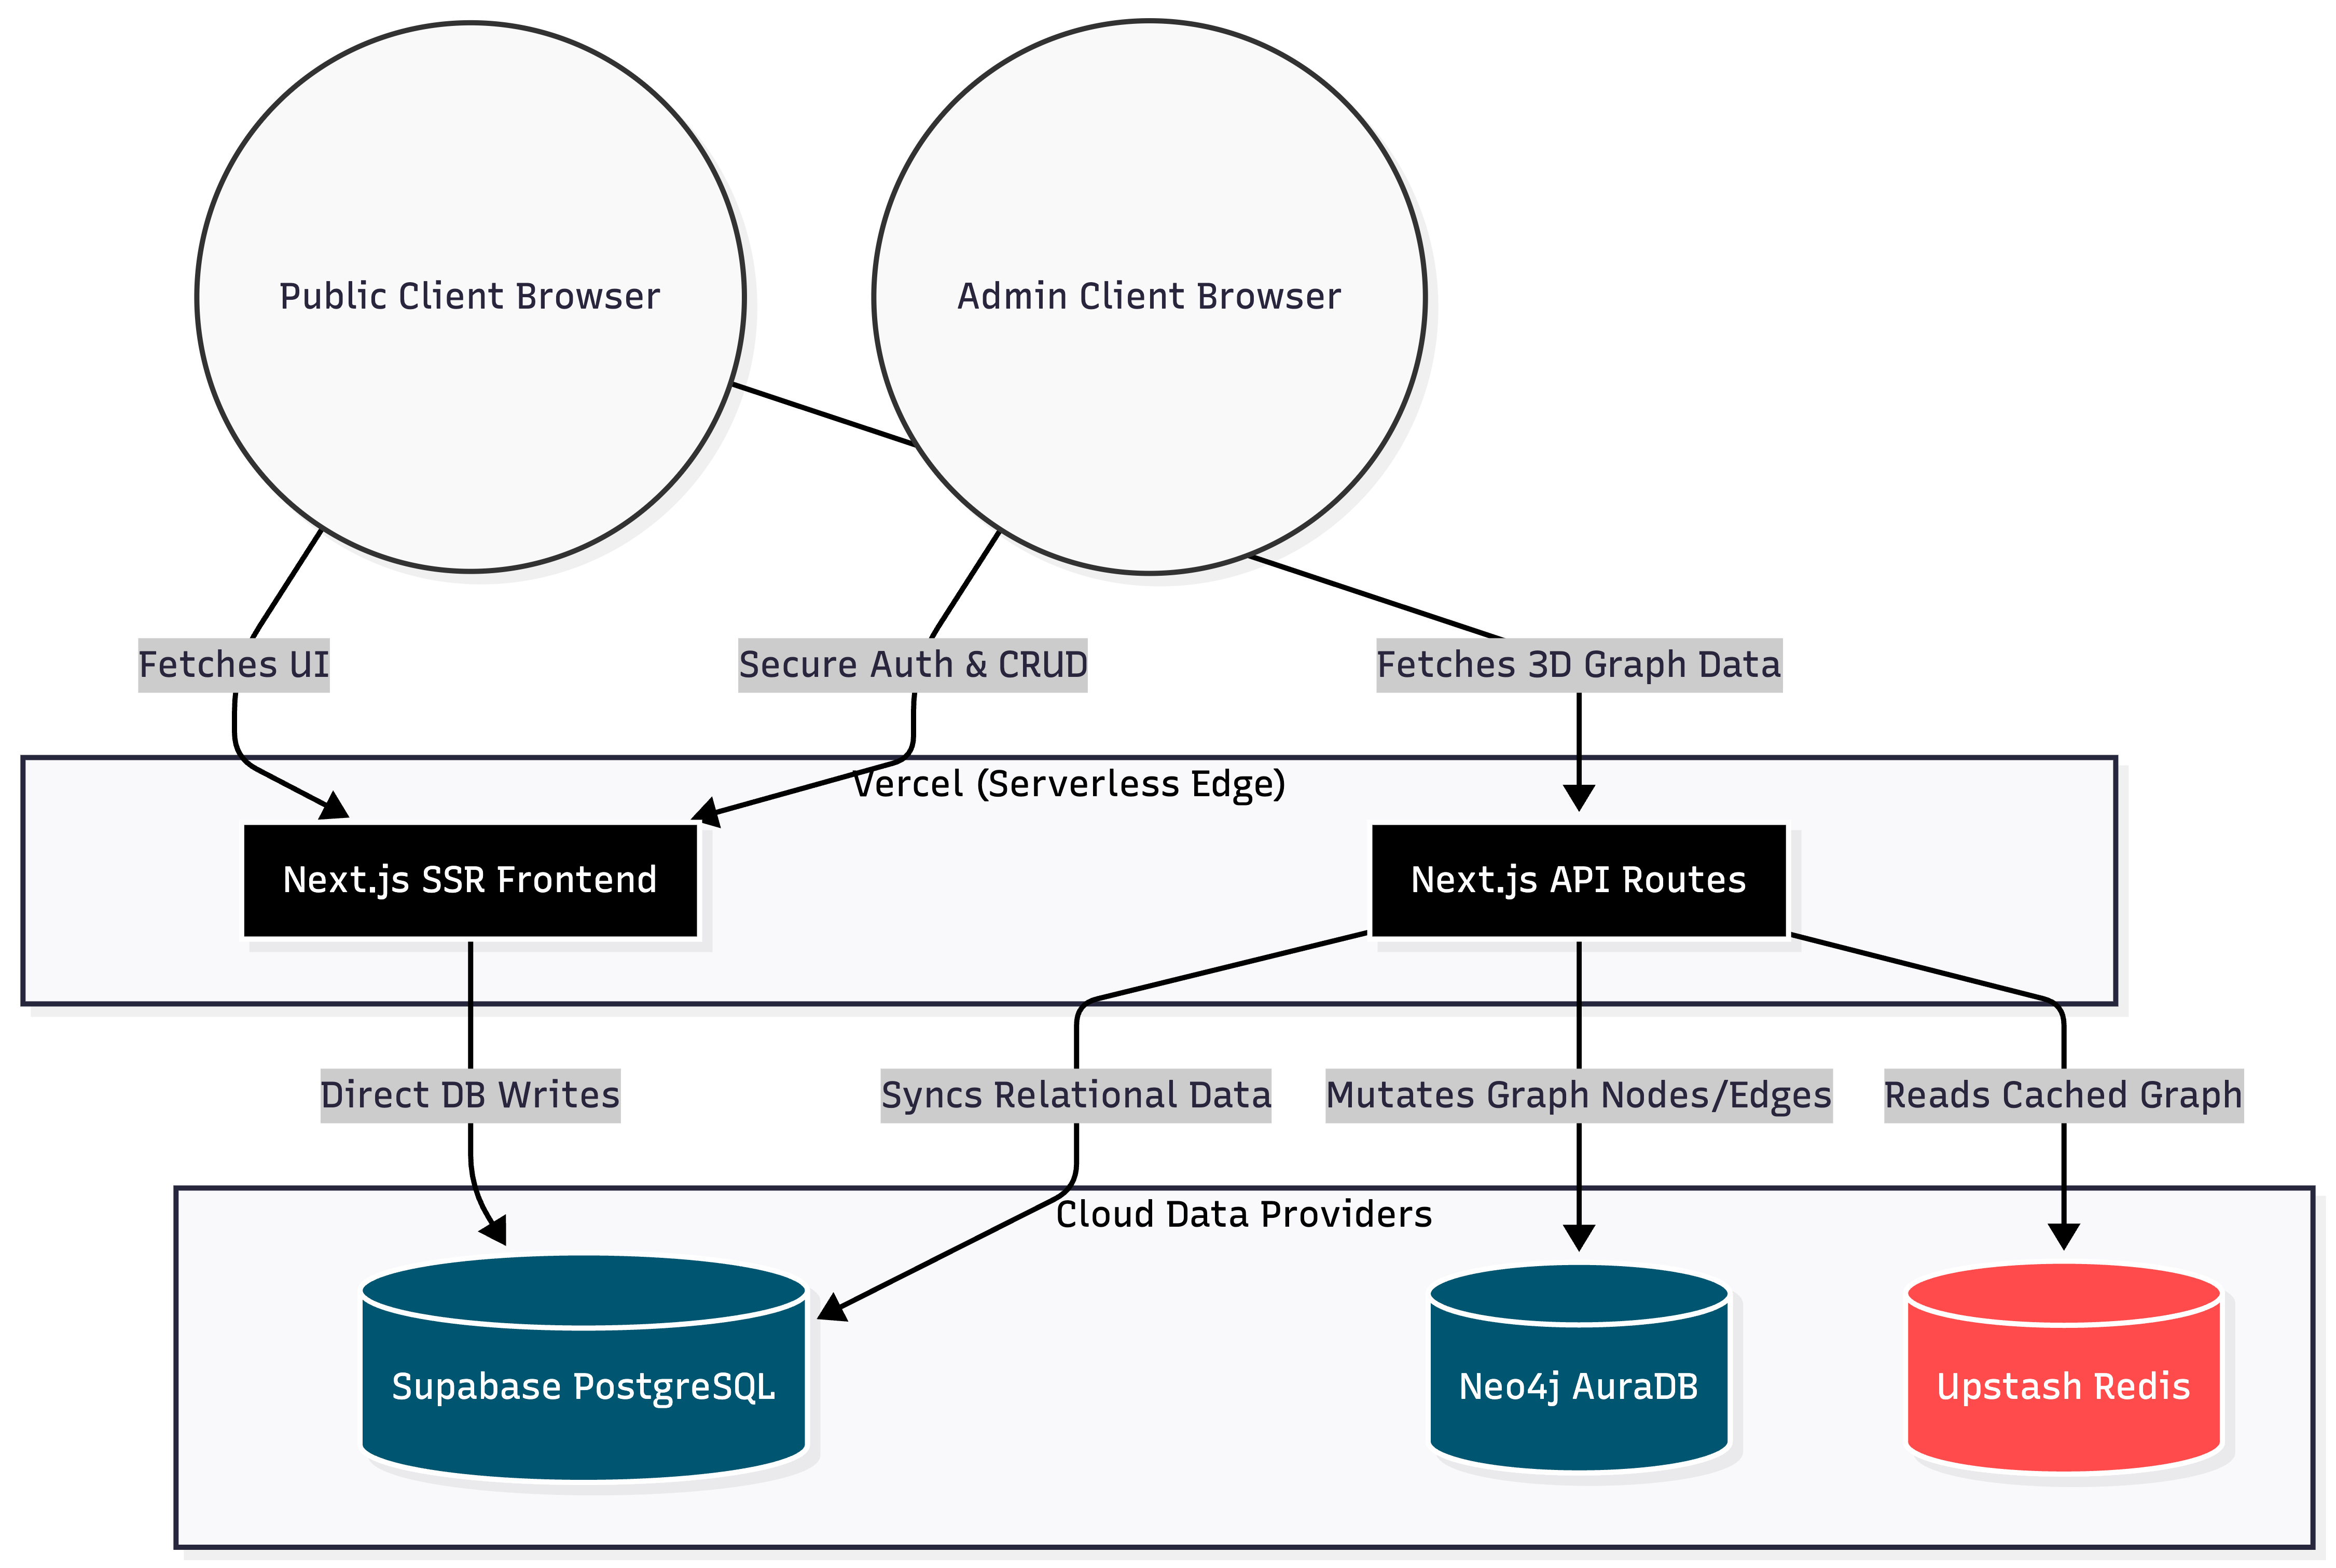
\includegraphics[width=0.7\textwidth]{images/deployment_diagram.png}
    \caption{Deployment Architecture Diagram}
    \label{fig:deployment}
\end{figure}

\section{System Models}

This section outlines the visual models used to understand and design the system's behavior and structure.

\subsection{Database Schema Diagrams}
This section visually outlines the structures of our two disparate data sources.

\subsubsection{Relational Model (Supabase/PostgreSQL)}
The Relational ERD focuses strictly on the core entities that support the graph model (\texttt{emcees}, \texttt{battles}, and \texttt{battle\_participants}). 

\begin{figure}[H]
    \centering
    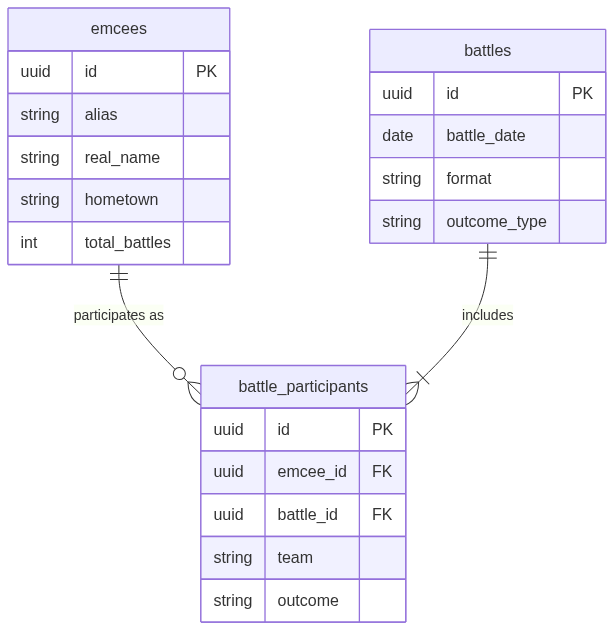
\includegraphics[width=0.9\textwidth]{images/supabase_erd.png}
    \caption{Relational Entity-Relationship Diagram (Supabase)}
    \label{fig:erd_supabase}
\end{figure}

\subsubsection{Property Graph Model (Neo4j)}
The Neo4j schema visualizes how the structured relational data is transformed into a node-edge network for traversal.

\begin{figure}[H]
    \centering
    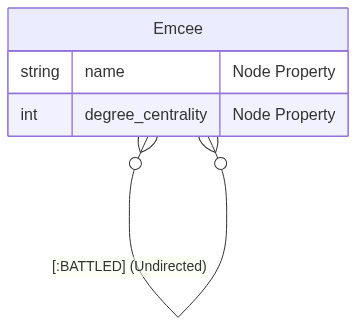
\includegraphics[width=0.8\textwidth]{images/neo4j_schema.png}
    \caption{Property Graph Model Schema (Neo4j)}
    \label{fig:erd_neo4j}
\end{figure}

\subsection{Unified Modeling Language (UML) Diagrams}

UML diagrams describe the behavioral and structural aspects of the fliptop.3d system.

\subsubsection{Use Case Diagram}
The Use Case Diagram defines the interactions between the system's actors (e.g., Public User, Administrator) and the system itself.

\begin{figure}[H]
    \centering
    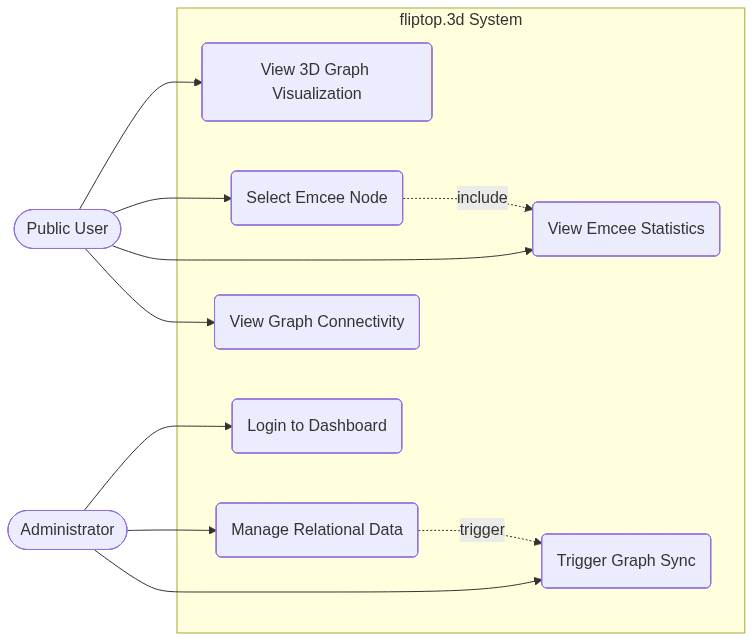
\includegraphics[width=1.0\textwidth]{images/use_case.png}
    \caption{Use Case Diagram}
    \label{fig:use_case}
\end{figure}

\subsubsection{Class Diagram}
The Class Diagram illustrates the object-oriented structure of the backend services and frontend components, particularly how the Next.js API routes interact with the Supabase client, Neo4j driver, and Upstash Redis.

\begin{figure}[H]
    \centering
    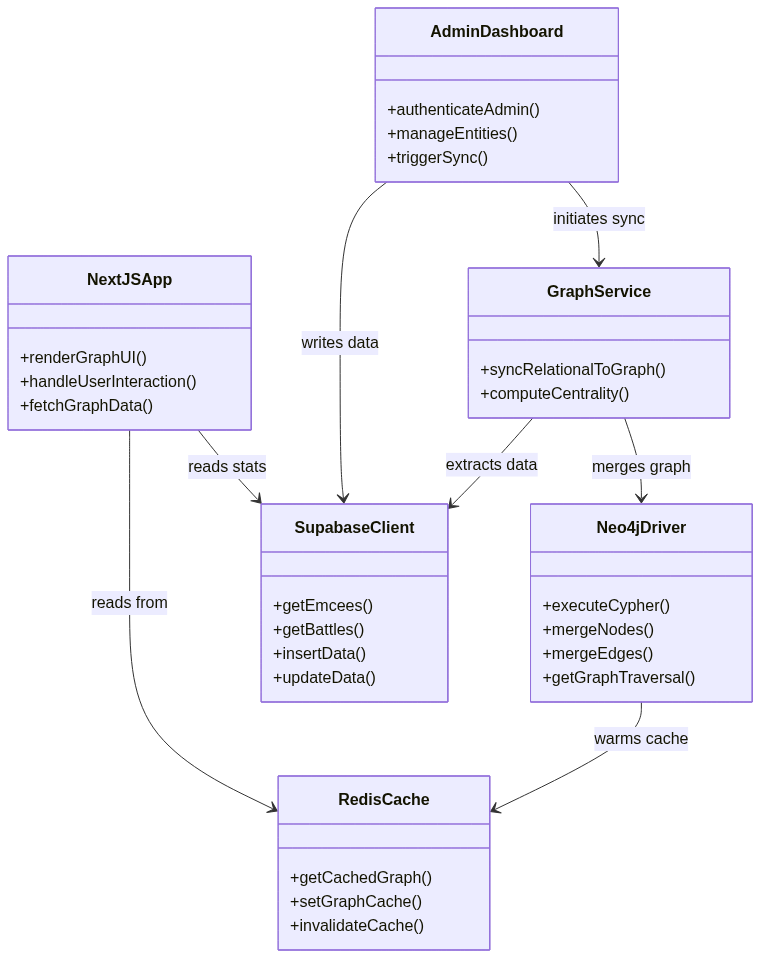
\includegraphics[width=1.0\textwidth]{images/class_diagram.png}
    \caption{Class Diagram}
    \label{fig:class_diagram}
\end{figure}

\subsubsection{Sequence Diagram}
The Sequence Diagram outlines the dynamic behavior and specific API calls involved when an Administrator synchronizes relational data (Supabase) to the graph model (Neo4j) and caches the result for the public client (Redis).

\begin{figure}[H]
    \centering
    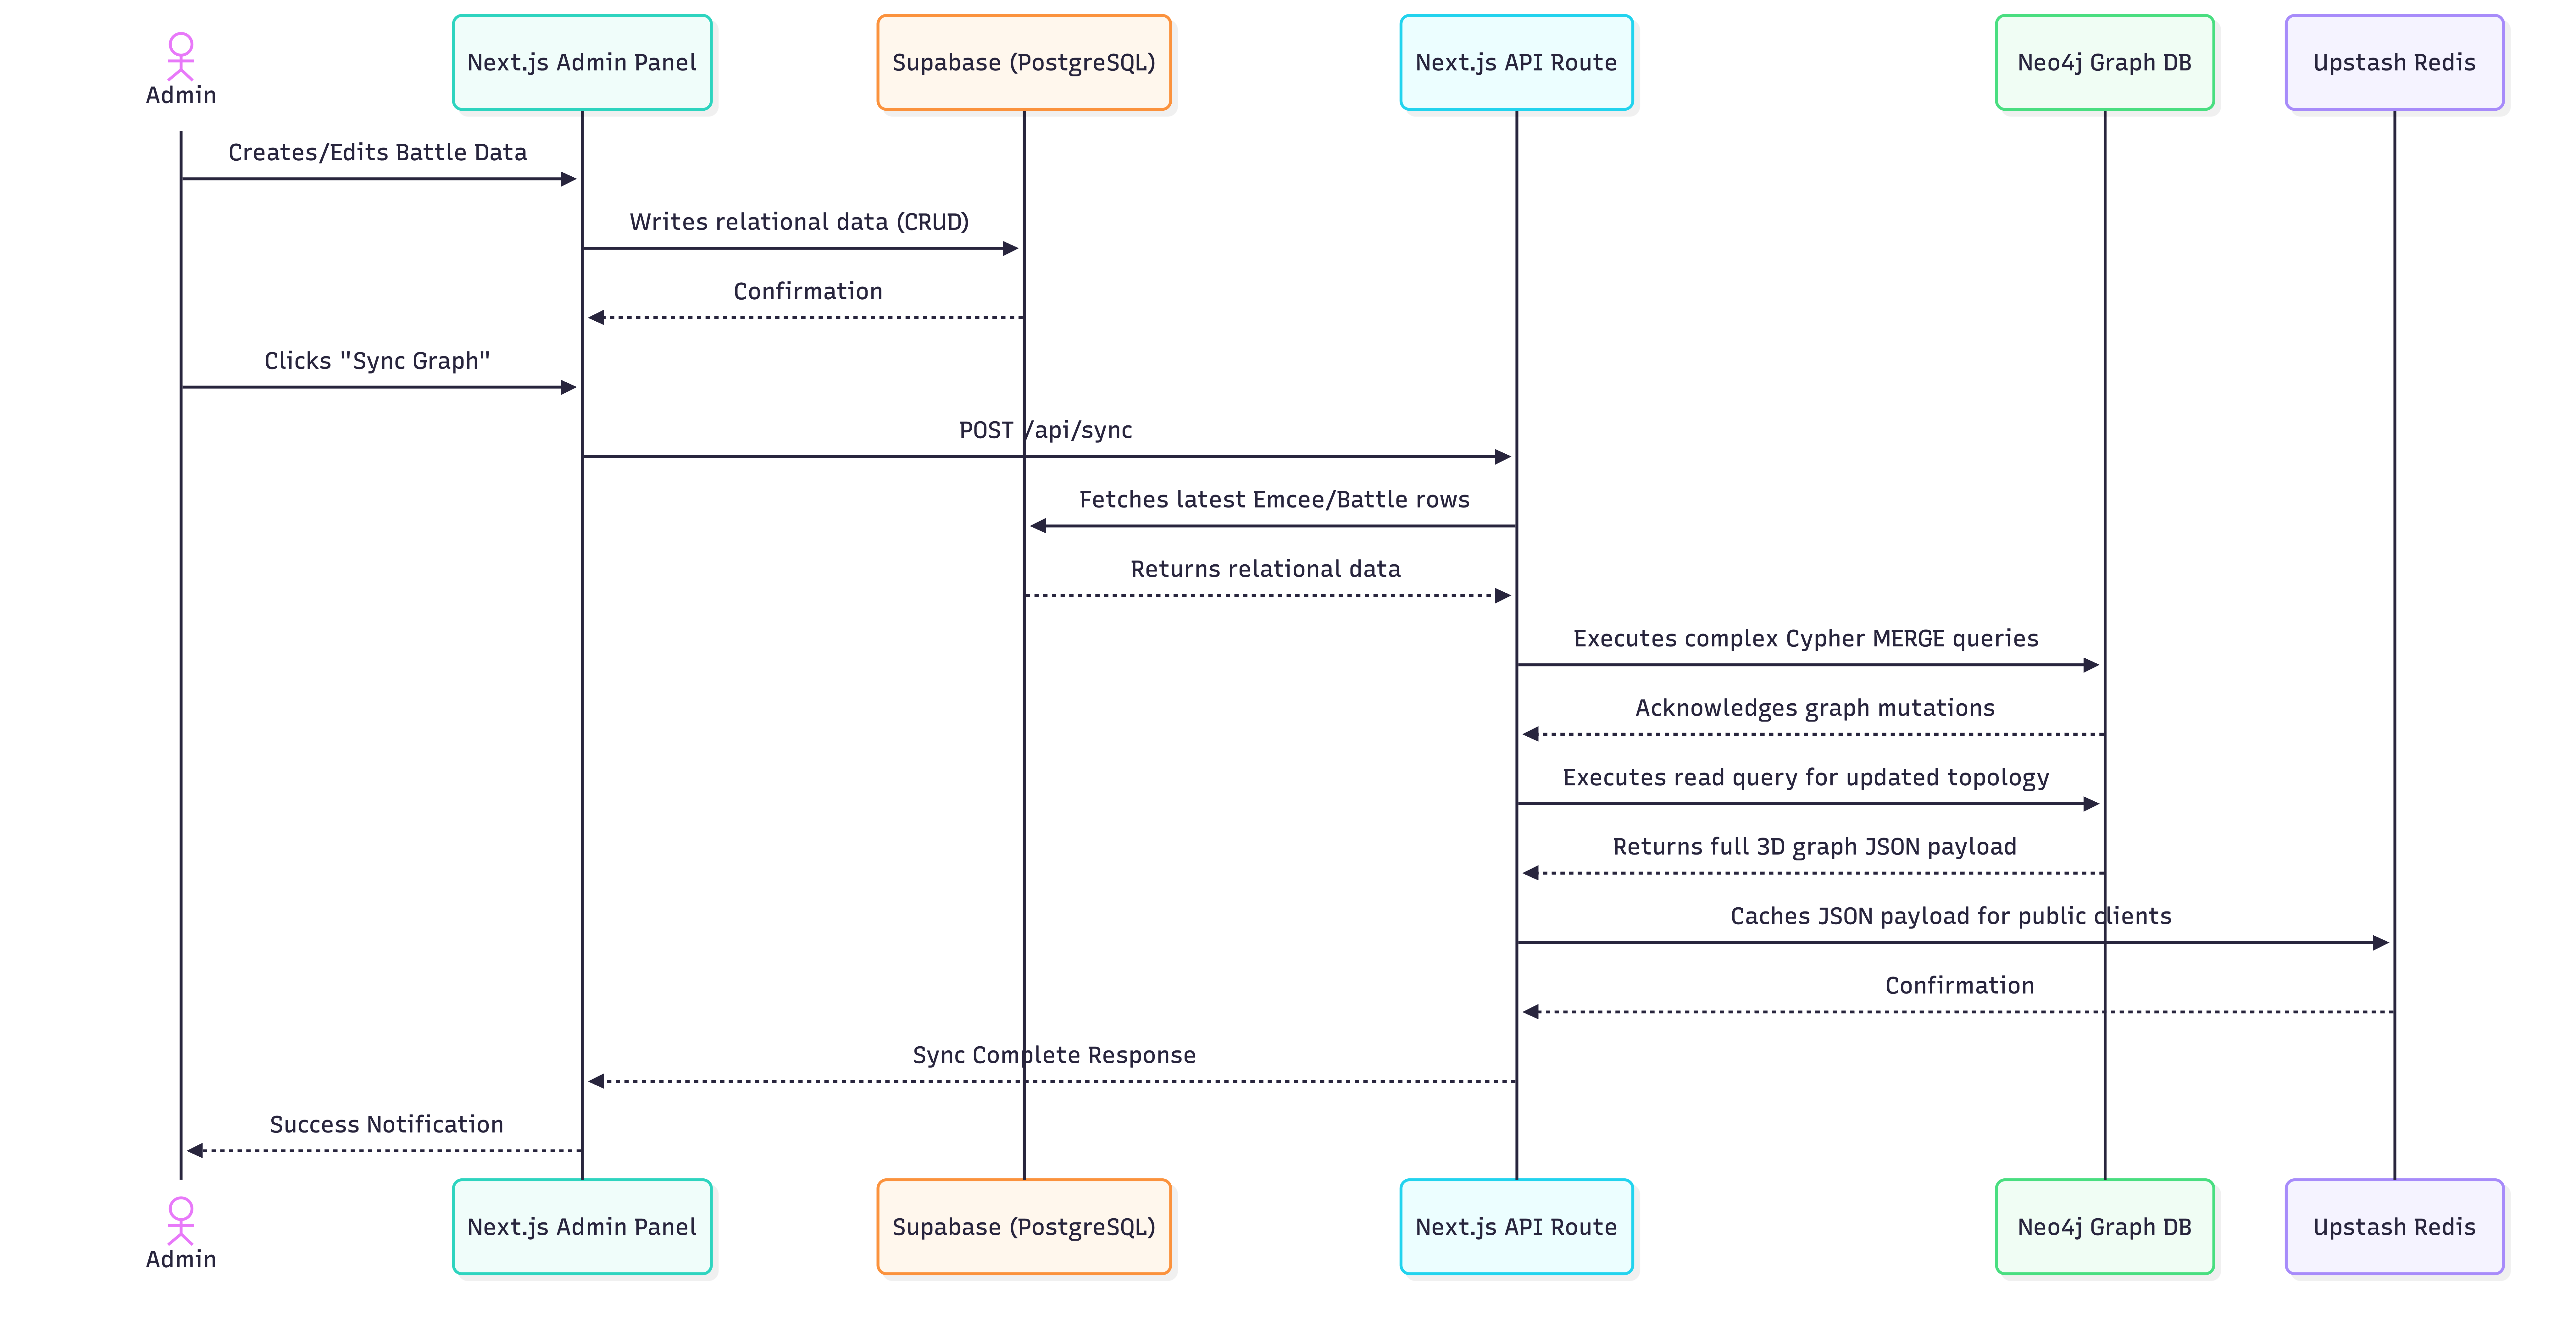
\includegraphics[width=0.85\textwidth]{images/sequence_diagram.png}
    \caption{Sequence Diagram (Data Synchronization Flow)}
    \label{fig:sequence}
\end{figure}

\subsection{Data Flow Diagram (DFD)}
The Data Flow Diagram tracks the movement of information through the system. Specifically, it highlights the CQRS pipeline: how an admin submits new battle data, how it is written to Supabase, how the synchronization routine pushes it to Neo4j, and how the client reads the cached graph data from Redis.

\begin{figure}[H]
    \centering
    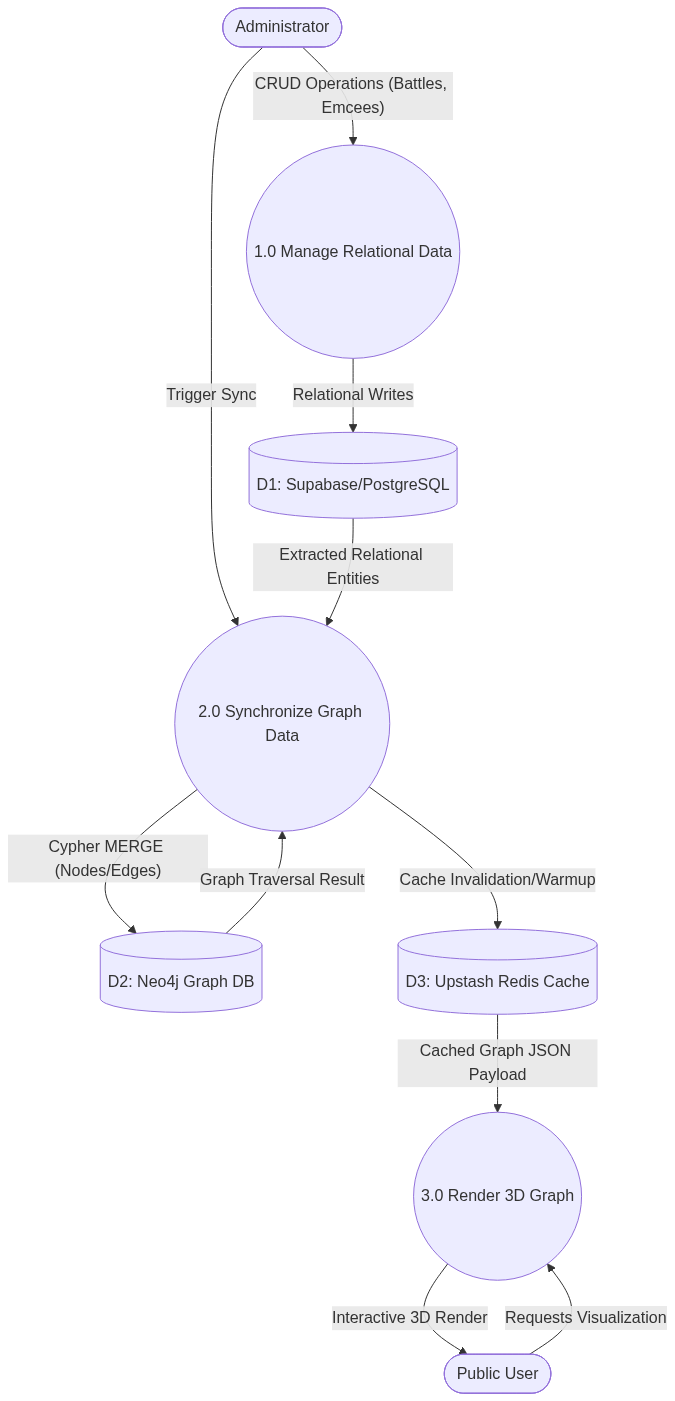
\includegraphics[width=0.8\textwidth,height=0.75\textheight,keepaspectratio]{images/dfd.png}
    \caption{Data Flow Diagram (Level 0/1)}
    \label{fig:dfd}
\end{figure}

\section{Database Design}

\subsection{Relational Model (Supabase/PostgreSQL)}
The relational database acts as the primary source of truth, structured in Third Normal Form (3NF) to ensure data integrity and prevent data anomalies. While the database contains numerous entities for media, events, and judging, the core schema that explicitly drives the graph visualization revolves around the following primary entities:

\begin{itemize}
    \item \textbf{Emcees (\texttt{emcees}):} The central entity representing individual battle rappers. It stores the unique identifier, alias, real name, and biographical metadata.
    \item \textbf{Battles (\texttt{battles}):} Stores individual matchup details. It tracks metadata like battle format and general outcomes.
    \item \textbf{Battle Participants (\texttt{battle\_participants}):} A crucial junction table resolving the many-to-many relationship between \texttt{emcees} and \texttt{battles}. It explicitly defines the role of the emcee in the battle and records their specific side or outcome in the matchup.
\end{itemize}

This normalized structure provides a highly structured, queryable foundation for the administrative backend, ensuring that the graph synchronization routines can seamlessly extract the \texttt{emcees} and their \texttt{battle\_participants} connections to generate the graph's nodes and edges.

\subsection{Graph Model (Neo4j)}
The graph database is highly optimized for read-heavy operations and UI rendering. The schema is strictly defined:
\begin{itemize}
    \item \textbf{Nodes:} Represent \texttt{Emcee} entities. Properties include name and degree (for centrality visualization).
    \item \textbf{Edges:} Represent relationships. 
    \begin{itemize}
        \item A \texttt{DEFEATED} edge is directed from the victor to the defeated.
        \item A \texttt{BATTLED} edge is bidirectional, representing a draw or an unjudged promotional match.
    \end{itemize}
\end{itemize}

\section{Subsystem and Interface Design}

\subsection{Interactive 3D Graph Rendering Module}
The primary user interface relies on WebGL mapping parsed graph data into a spatial physics-based layout.
\begin{itemize}
    \item \textbf{Degree Centrality Visualization:} The rendering algorithm dynamically scales node sizes based on an Emcee's total number of edges (battle count). This instantly visually distinguishes veteran participants from newcomers.
    \item \textbf{Node-Specific Subgraph Highlighting:} Selecting a node triggers a UI overlay containing the Emcee's aggregated statistics and dims all unrelated edges in the 3D space. This interaction emphasizes the selected entity's direct battle network.
\end{itemize}

\subsection{Administrative Synchronization Module}
A secure dashboard is provided for data management. It allows administrators to perform CRUD operations directly on the relational database. Subsequently, users can trigger synchronization routines that map the relational data into graph structures using complex Cypher \texttt{MERGE} operations to ensure idempotency.

\section{User Interface \& Experience (UI/UX)}

The system's UI is designed with a dark-mode aesthetic to emphasize the vibrant colors of the 3D graph nodes and edges. The interface is intentionally minimalist to prevent cognitive overload, allowing the spatial data to be the focal point of the user experience.

\subsection{Visual Legend \& Symbology}
To effectively communicate the complex data within the 3D space, the system employs a strict visual legend:
\begin{itemize}
    \item \textbf{Node Colors (Win Rate):} An Emcee's node color operates on an HSL spectrum mapping their career Win Rate. A 0\% win rate renders as \textbf{Red}, a 50\% win rate as \textbf{Yellow}, and a 100\% win rate as \textbf{Green}.
    \item \textbf{Edge Colors (Match Types):} Links between nodes are color-coded by the event format:
    \begin{itemize}
        \item \textbf{Metallic Gold:} Official Tournament Matches.
        \item \textbf{Slate Grey:} Standard Judged Battles.
        \item \textbf{Magenta:} Promotional Matches.
        \item \textbf{Blue:} Tryout Matches.
    \end{itemize}
    \item \textbf{Directional Particles:} Animated light particles travel along the edges to represent outcomes. In standard unselected views, \textbf{Gold} particles continuously flow along Tournament edges. When a specific Emcee node is selected, particles flow rapidly along their connecting edges: \textbf{Green particles} flowing inward represent a victory for the selected Emcee, while \textbf{Red particles} flowing outward represent a defeat.
\end{itemize}

\begin{figure}[H]
    \centering
    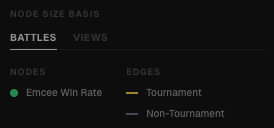
\includegraphics[width=0.35\textwidth,height=0.25\textheight,keepaspectratio]{images/tools/legend.png}
    \caption{On-Screen Visual Legend (Browser: Chrome 149, OS: Mac OS Sonoma)}
    \label{fig:ui_legend}
\end{figure}

\subsection{System Functionalities}
The application features several dynamic interactive capabilities for exploring the graph:
\begin{itemize}
    \item \textbf{Dynamic Node Sizing:} Node sizes can be toggled to scale by the total number of \textit{battles} an emcee has participated in, or by their total accumulated \textit{views}.
    \item \textbf{Temporal Filtering:} Users can filter nodes by specific years. By default, the system displays \textit{All Years}, rendering all nodes alongside both tournament and non-tournament links.
\end{itemize}

\subsection{Interactive Controls \& Navigation}
The floating control menu allows rapid manipulation of the graph's rendering parameters.

\begin{figure}[H]
    \centering
    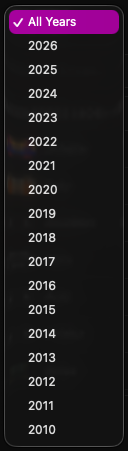
\includegraphics[width=0.25\textwidth,height=0.15\textheight,keepaspectratio]{images/tools/year-dropdown.png}
    \hspace{0.05\textwidth}
    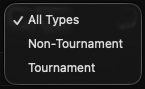
\includegraphics[width=0.25\textwidth,height=0.15\textheight,keepaspectratio]{images/tools/battle-type-dropdown.png}
    \caption{Temporal and Match Type Filters (Browser: Chrome 149, OS: Mac OS Sonoma)}
    \label{fig:ui_dropdowns}
\end{figure}

\begin{figure}[H]
    \centering
    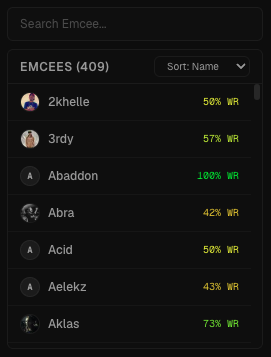
\includegraphics[width=0.35\textwidth,height=0.25\textheight,keepaspectratio]{images/tools/emcee-filter.png}
    \caption{Emcee Search and Sort Panel (Browser: Chrome 149, OS: Mac OS Sonoma)}
    \label{fig:ui_emcee_filter}
\end{figure}

\subsection{Core Visualization Interface}
The core screen occupies the full viewport, rendering the WebGL canvas with interactive graph filters and overlay panels.

\begin{figure}[H]
    \centering
    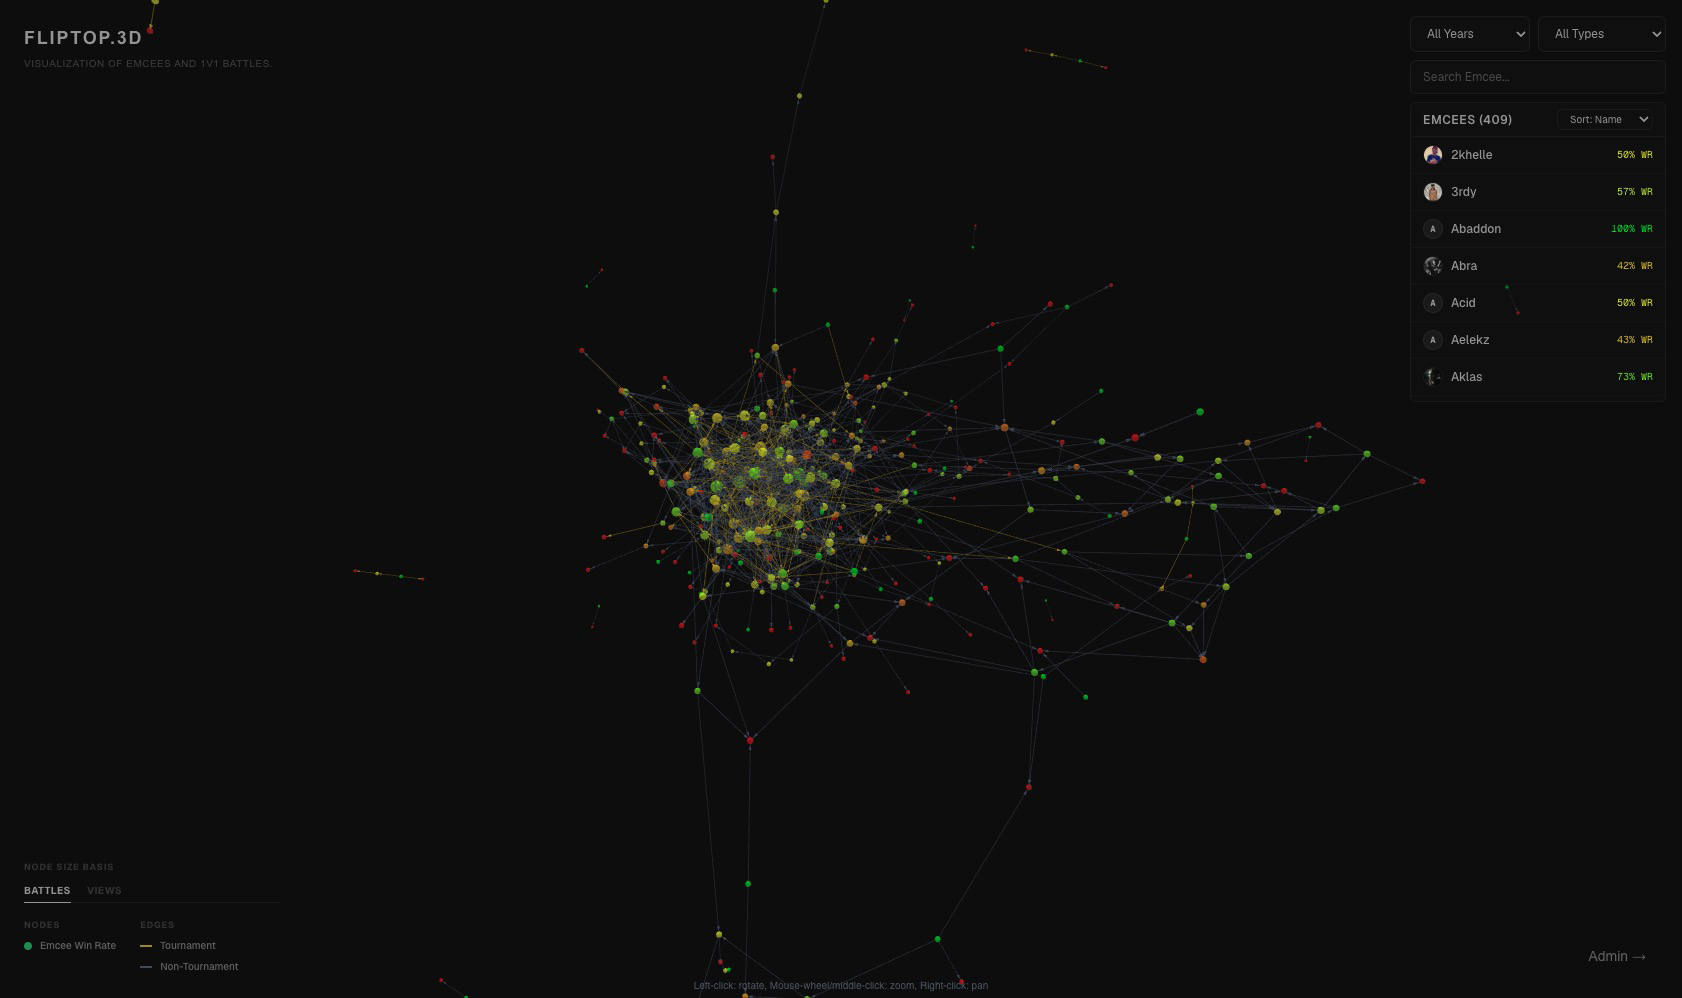
\includegraphics[width=0.9\textwidth,height=0.45\textheight,keepaspectratio]{images/home.png}
    \caption{Default Home View showing all years and link types (Browser: Chrome 149, OS: Mac OS Sonoma)}
    \label{fig:ui_home}
\end{figure}

\begin{figure}[H]
    \centering
    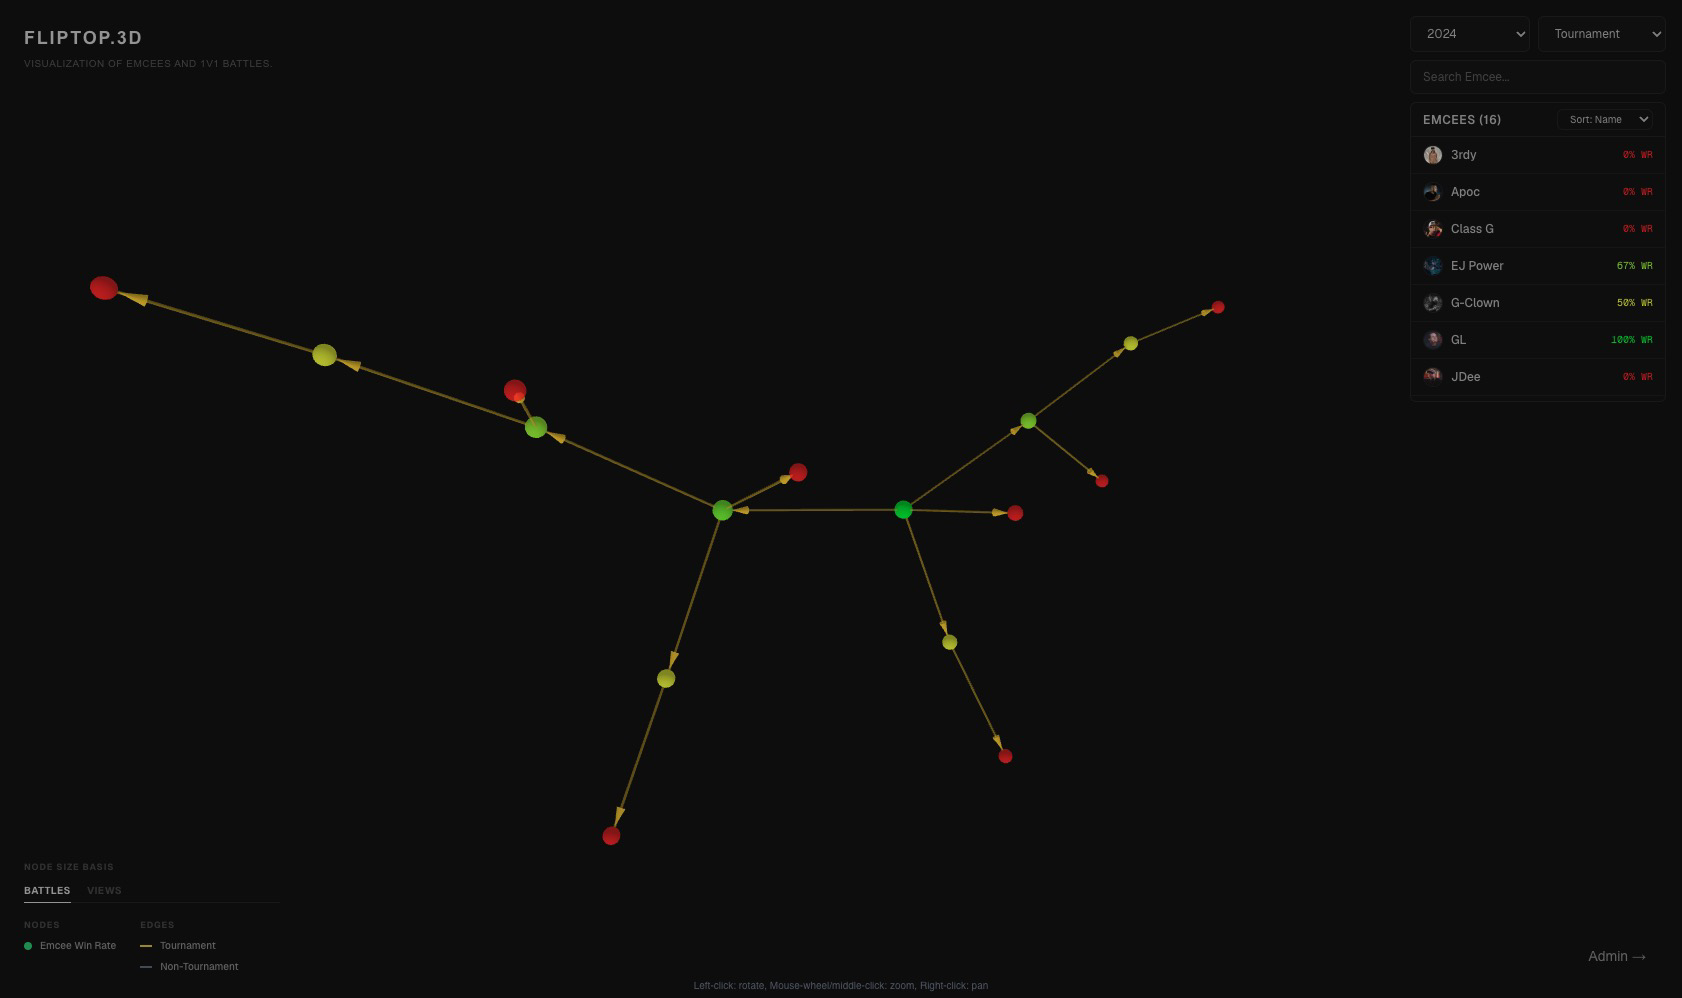
\includegraphics[width=0.9\textwidth,height=0.45\textheight,keepaspectratio]{images/2024_nodes-by-battles.png}
    \caption{Graph filtered by Year 2024 with nodes sized by Total Battles (Browser: Chrome 149, OS: Mac OS Sonoma)}
    \label{fig:ui_2024_battles}
\end{figure}

\begin{figure}[H]
    \centering
    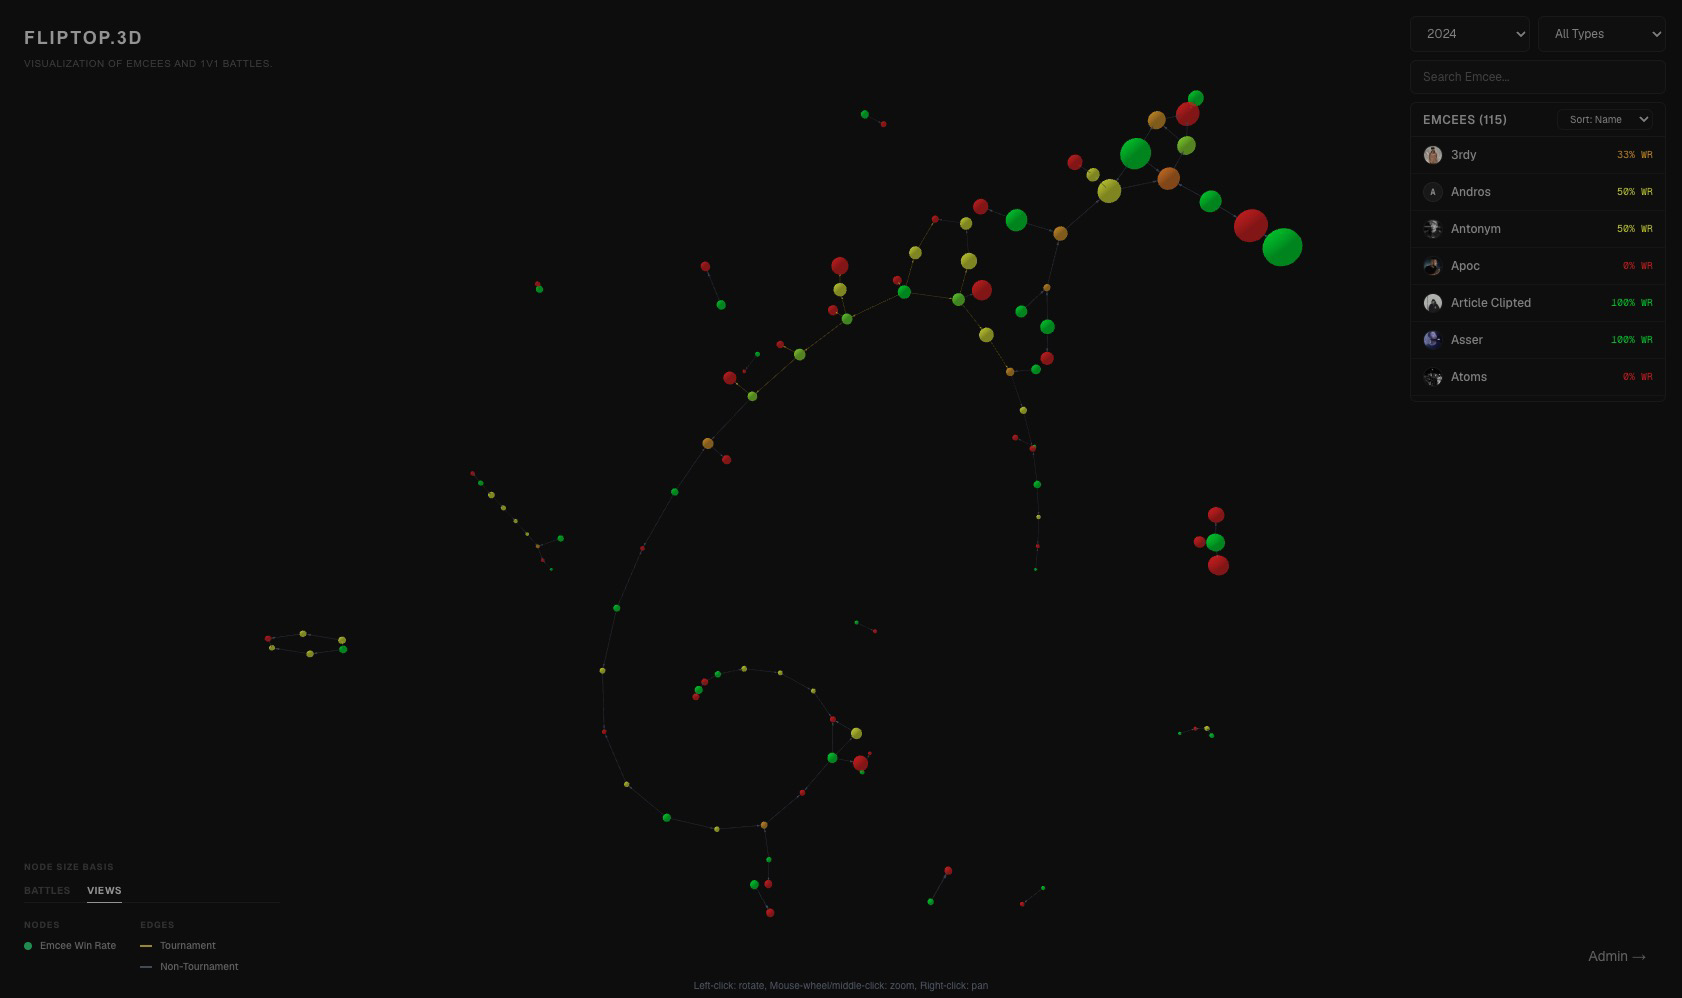
\includegraphics[width=0.9\textwidth,height=0.45\textheight,keepaspectratio]{images/2024_nodes-by-views.png}
    \caption{Graph filtered by Year 2024 with nodes sized by Total Views (Browser: Chrome 149, OS: Mac OS Sonoma)}
    \label{fig:ui_2024_views}
\end{figure}

\subsection{Interactive Overlays}
Selecting specific entities triggers a UI overlay containing aggregated statistics while keeping the graph context visible.

\begin{figure}[H]
    \centering
    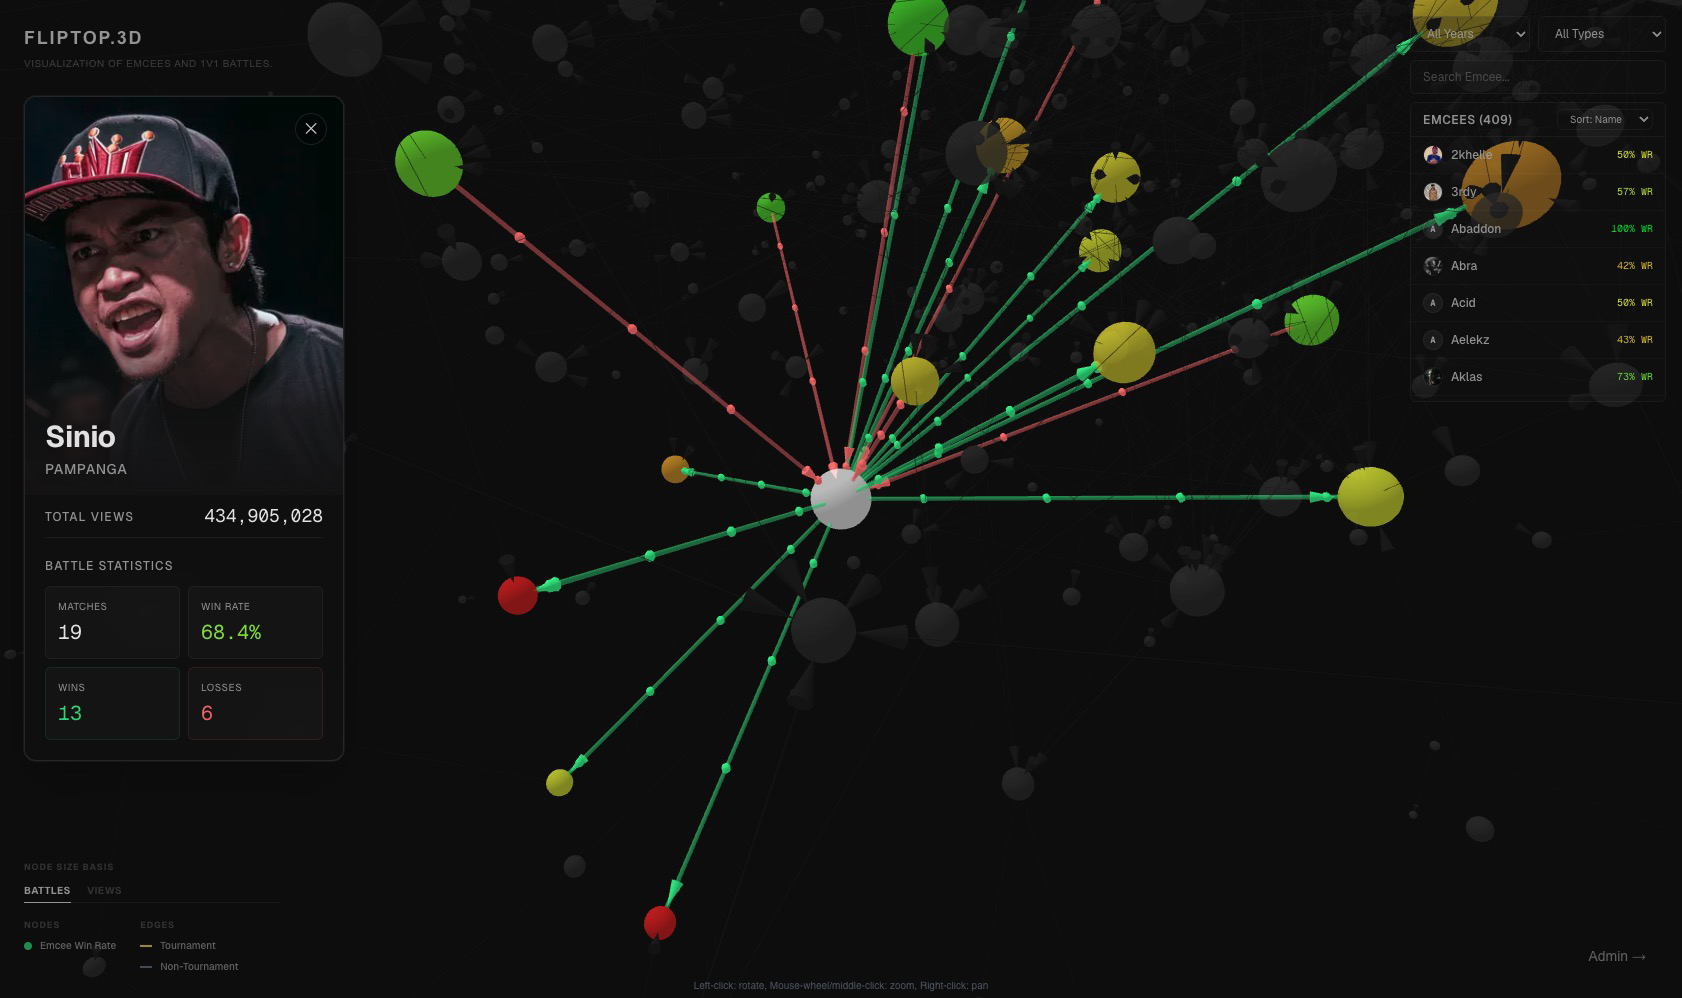
\includegraphics[width=0.9\textwidth,height=0.45\textheight,keepaspectratio]{images/emcee.png}
    \caption{Emcee Node Selection Overlay (Browser: Chrome 149, OS: Mac OS Sonoma)}
    \label{fig:ui_emcee}
\end{figure}

\begin{figure}[H]
    \centering
    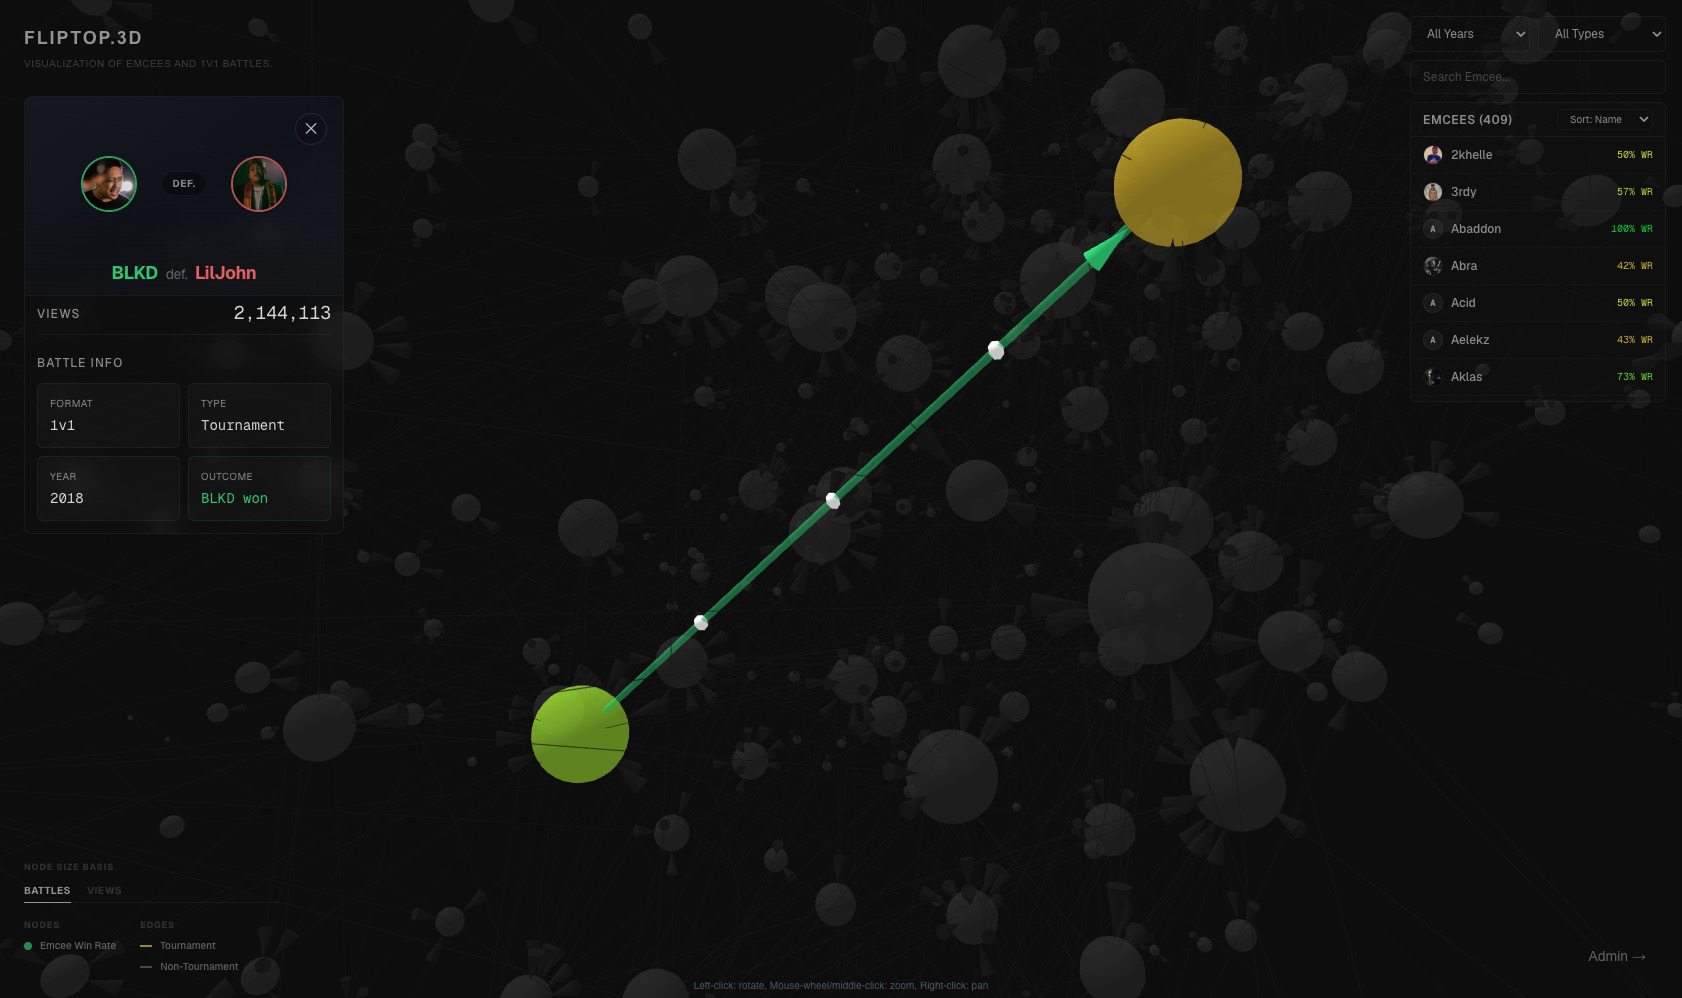
\includegraphics[width=0.9\textwidth,height=0.45\textheight,keepaspectratio]{images/battle.png}
    \caption{Battle Selection Overlay (Browser: Chrome 149, OS: Mac OS Sonoma)}
    \label{fig:ui_battle}
\end{figure}

\subsection{Mobile Responsiveness \& Interface}
The application is fully responsive, ensuring the 3D graph visualization and core interactions remain accessible on mobile devices. Note that administrative capabilities are restricted to desktop environments; there is no admin dashboard access provided on mobile devices to ensure data integrity and prevent accidental CRUD operations on smaller touch screens.

\begin{figure}[H]
    \centering
    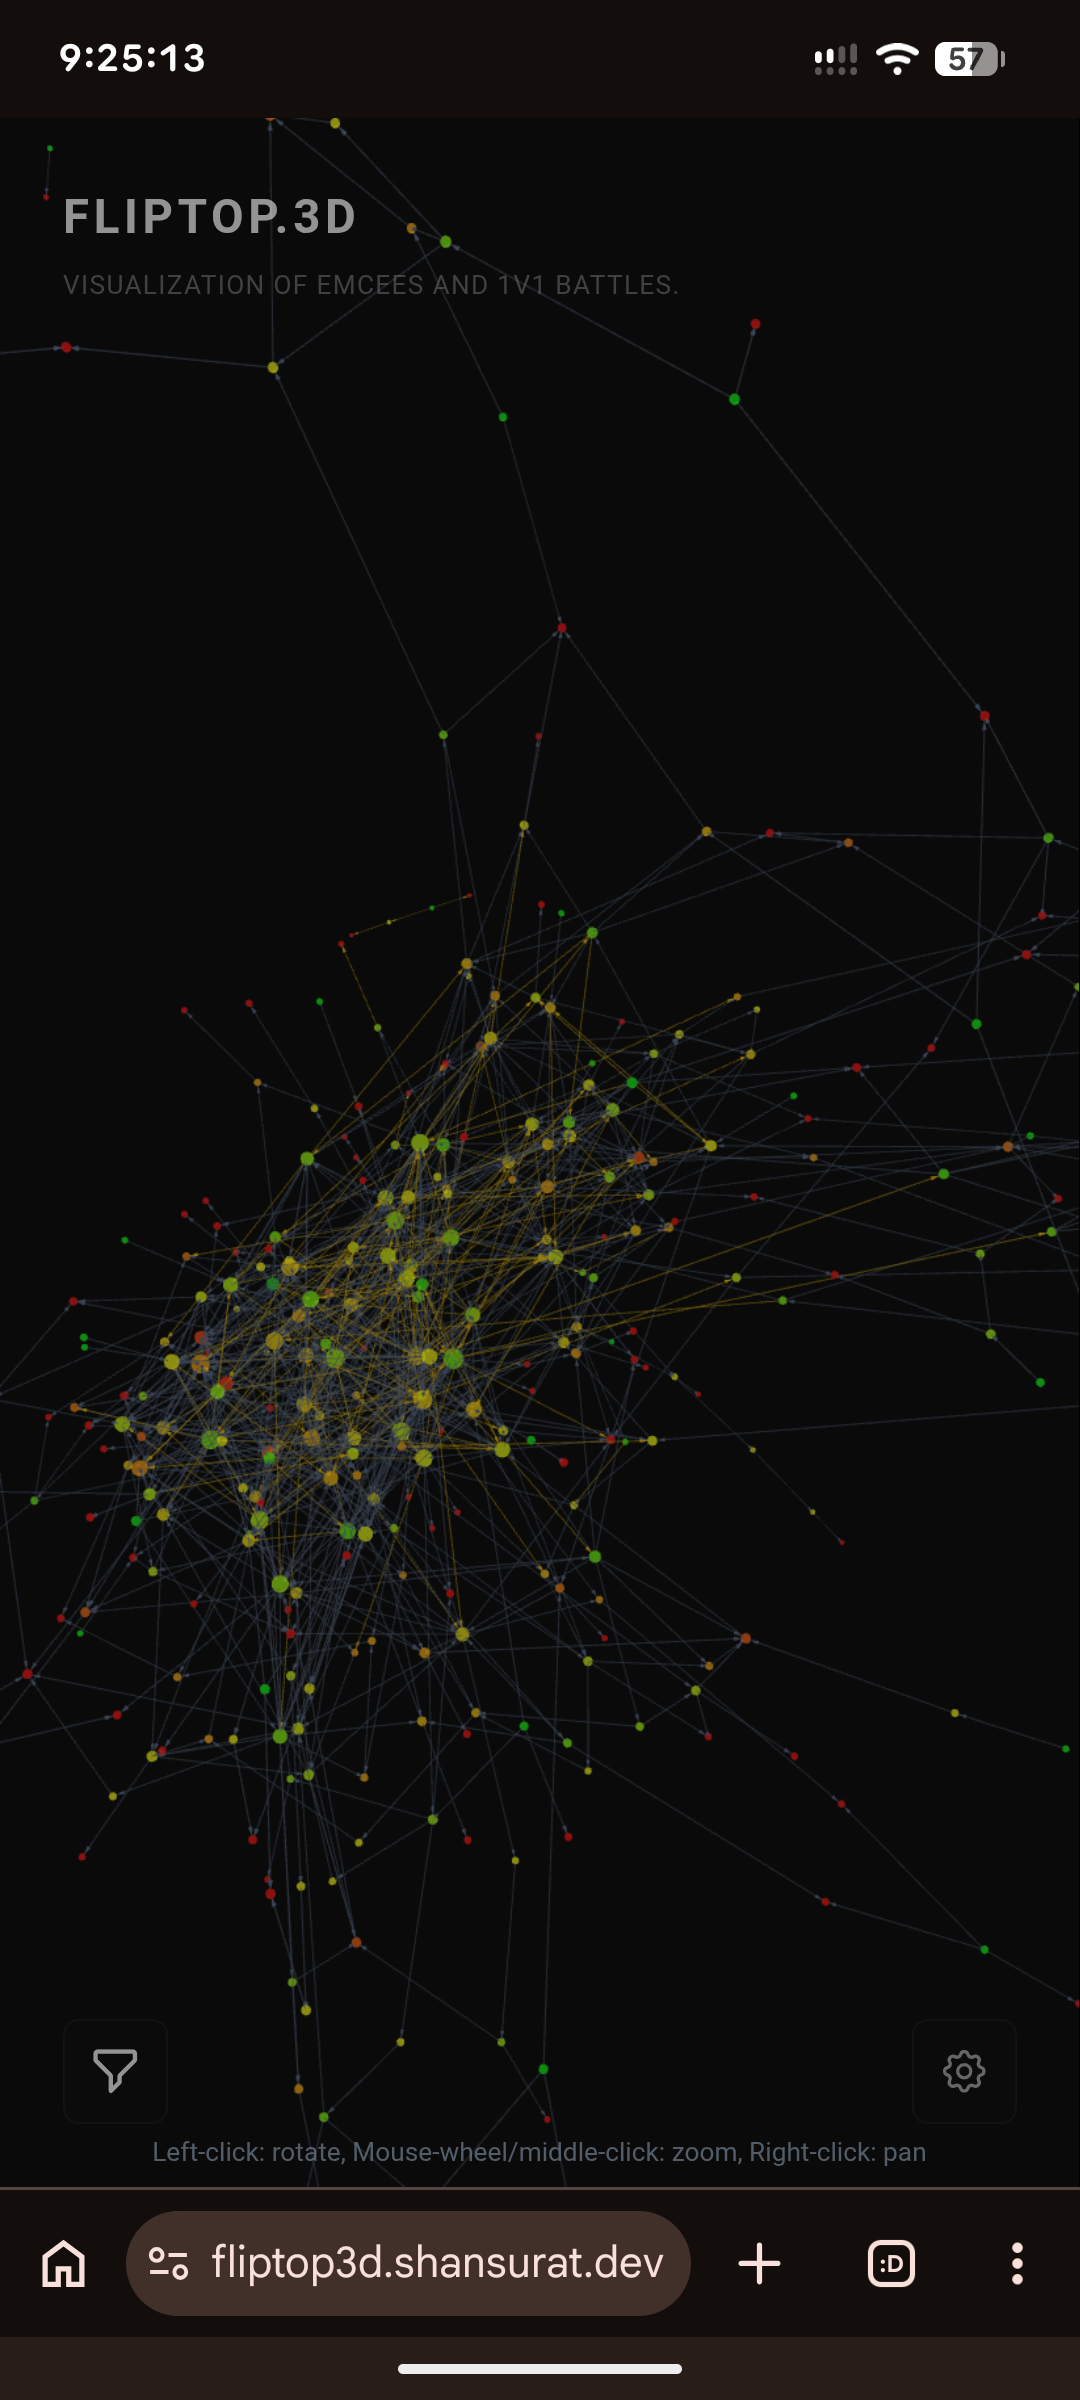
\includegraphics[width=0.3\textwidth]{images/tools/mobile/Screenshot_20260607-092514.png}
    \hspace{0.02\textwidth}
    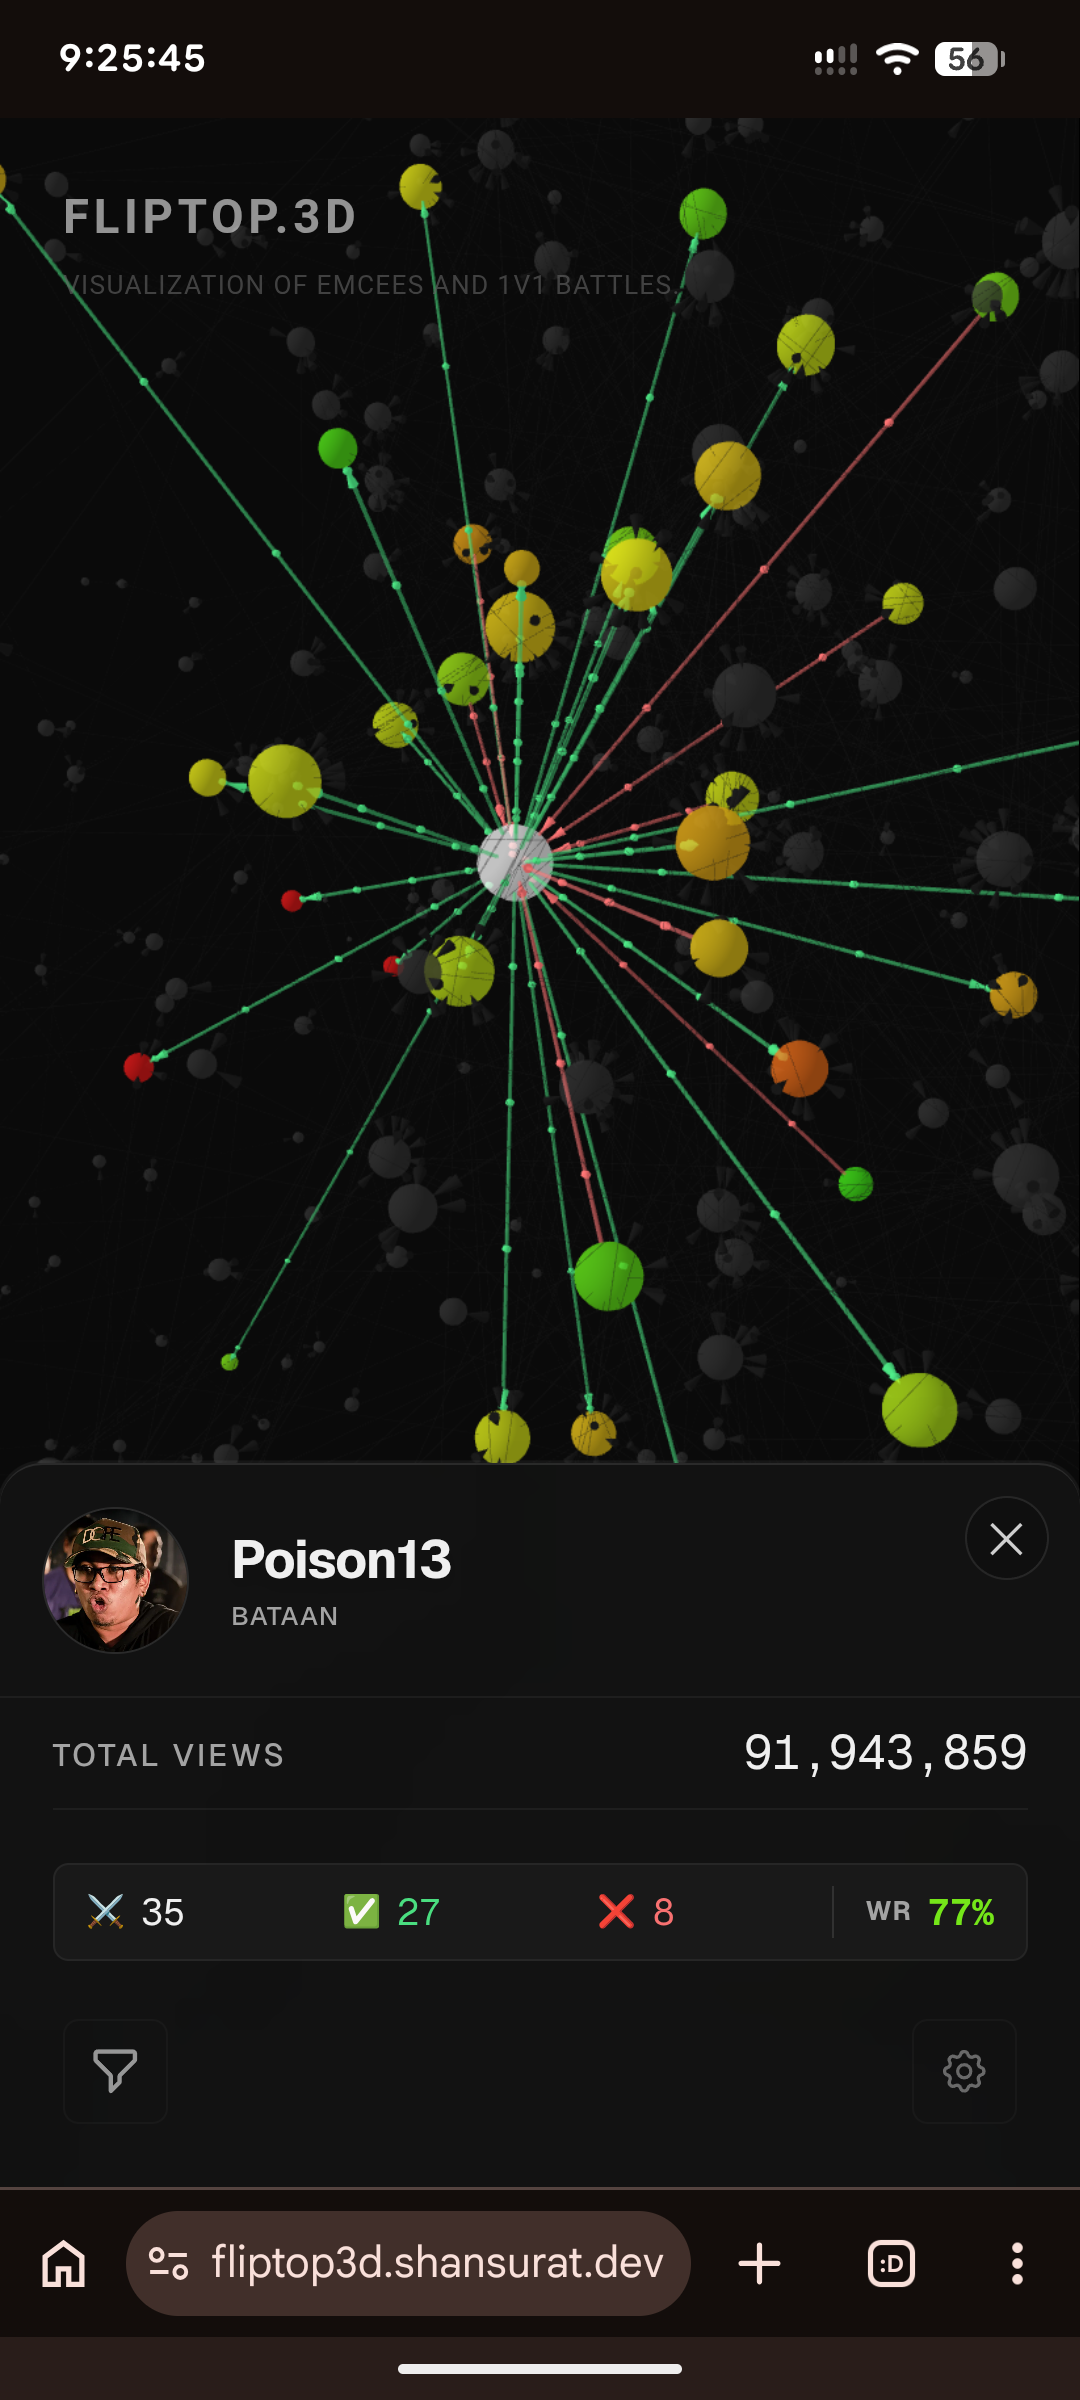
\includegraphics[width=0.3\textwidth]{images/tools/mobile/Screenshot_20260607-092546.png}
    \hspace{0.02\textwidth}
    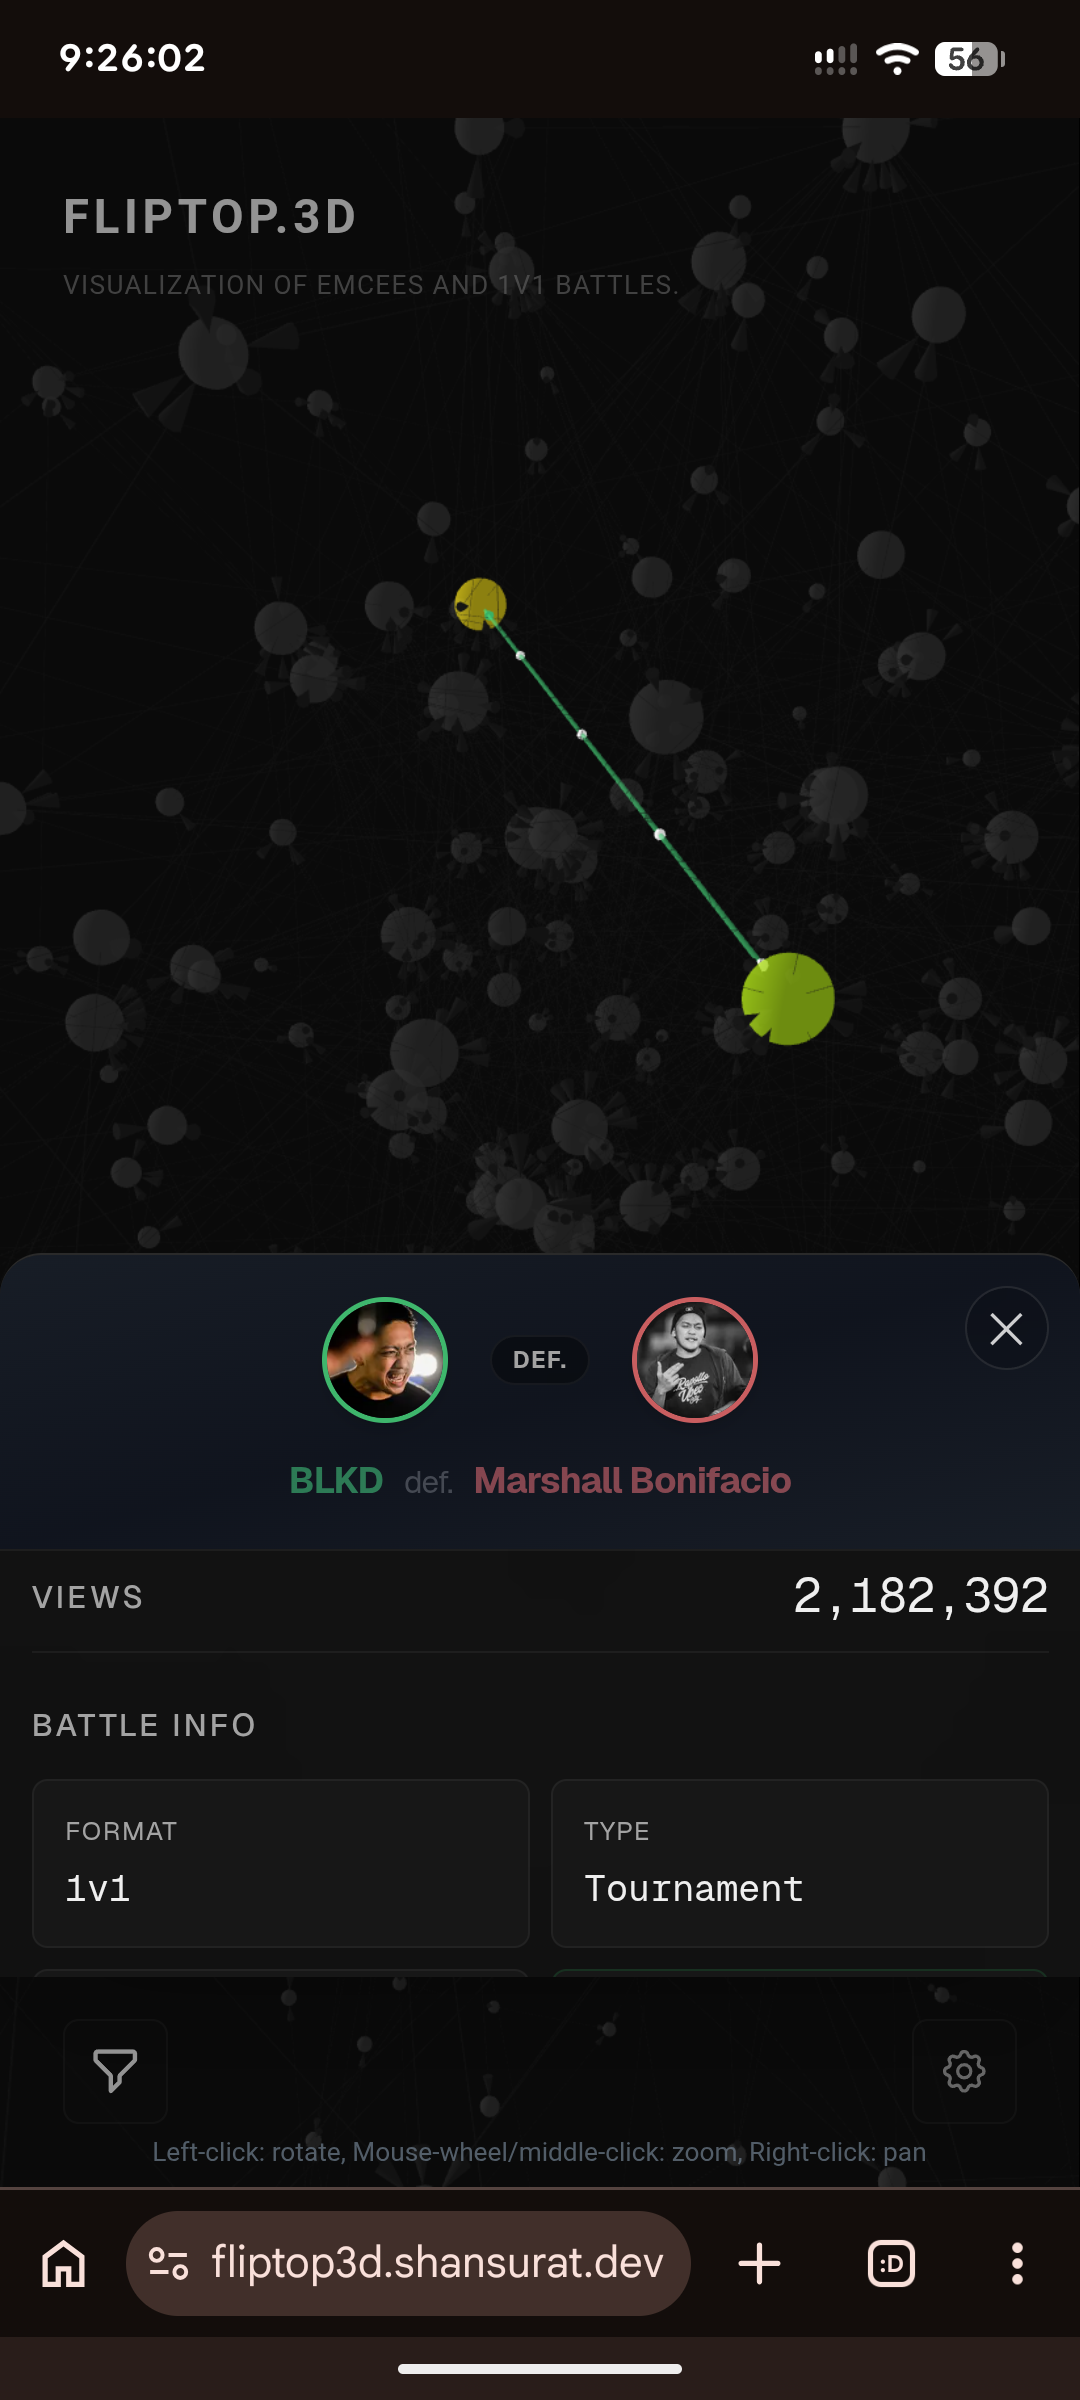
\includegraphics[width=0.3\textwidth]{images/tools/mobile/Screenshot_20260607-092603.png}
    \caption{Mobile Interface Views (Browser: Chrome 149, OS: Android, Device: Pixel 7A)}
    \label{fig:ui_mobile}
\end{figure}

\subsection{Administrative Dashboard}
The secure dashboard utilizes traditional tabular layouts optimized for CRUD operations, providing administrators with high-density data views for rapid editing. Access to this subsystem is heavily gated by an authentication layer and is strictly restricted to desktop environments (mobile access is disabled).

\begin{figure}[H]
    \centering
    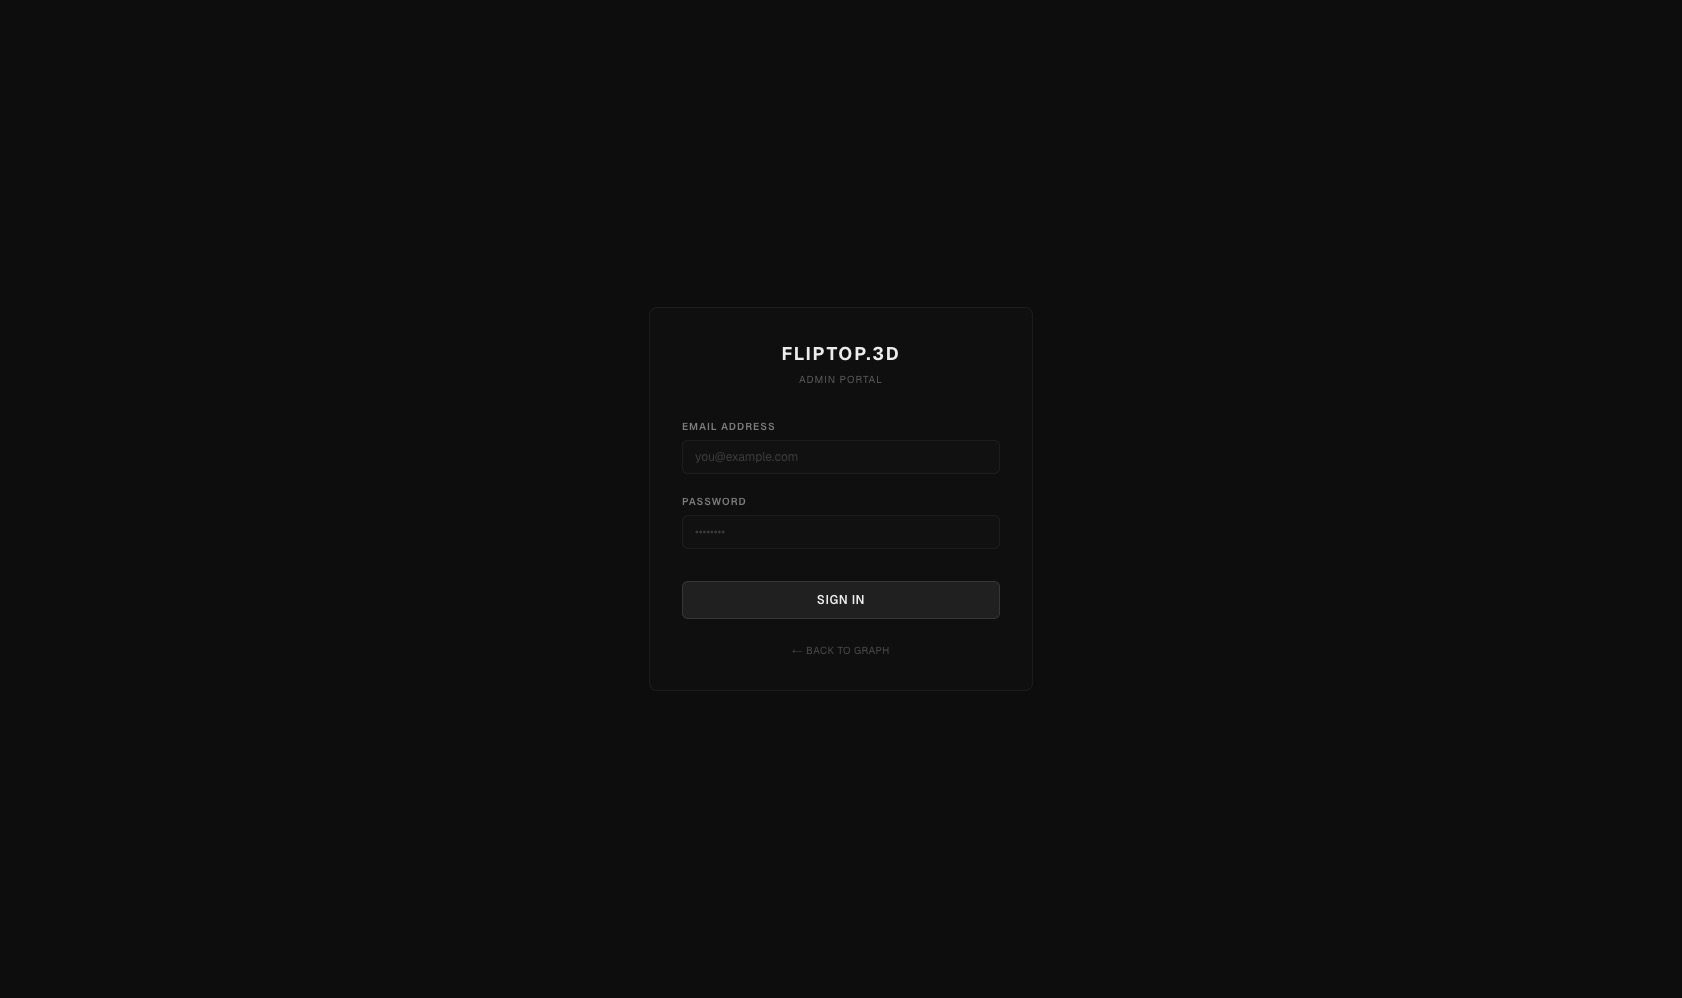
\includegraphics[width=0.8\textwidth,height=0.25\textheight,keepaspectratio]{images/auth.png}
    \caption{Administrative Secure Login Gateway (Browser: Chrome 149, OS: Mac OS Sonoma)}
    \label{fig:ui_admin_auth}
    
    \vspace{0.5cm}
    
    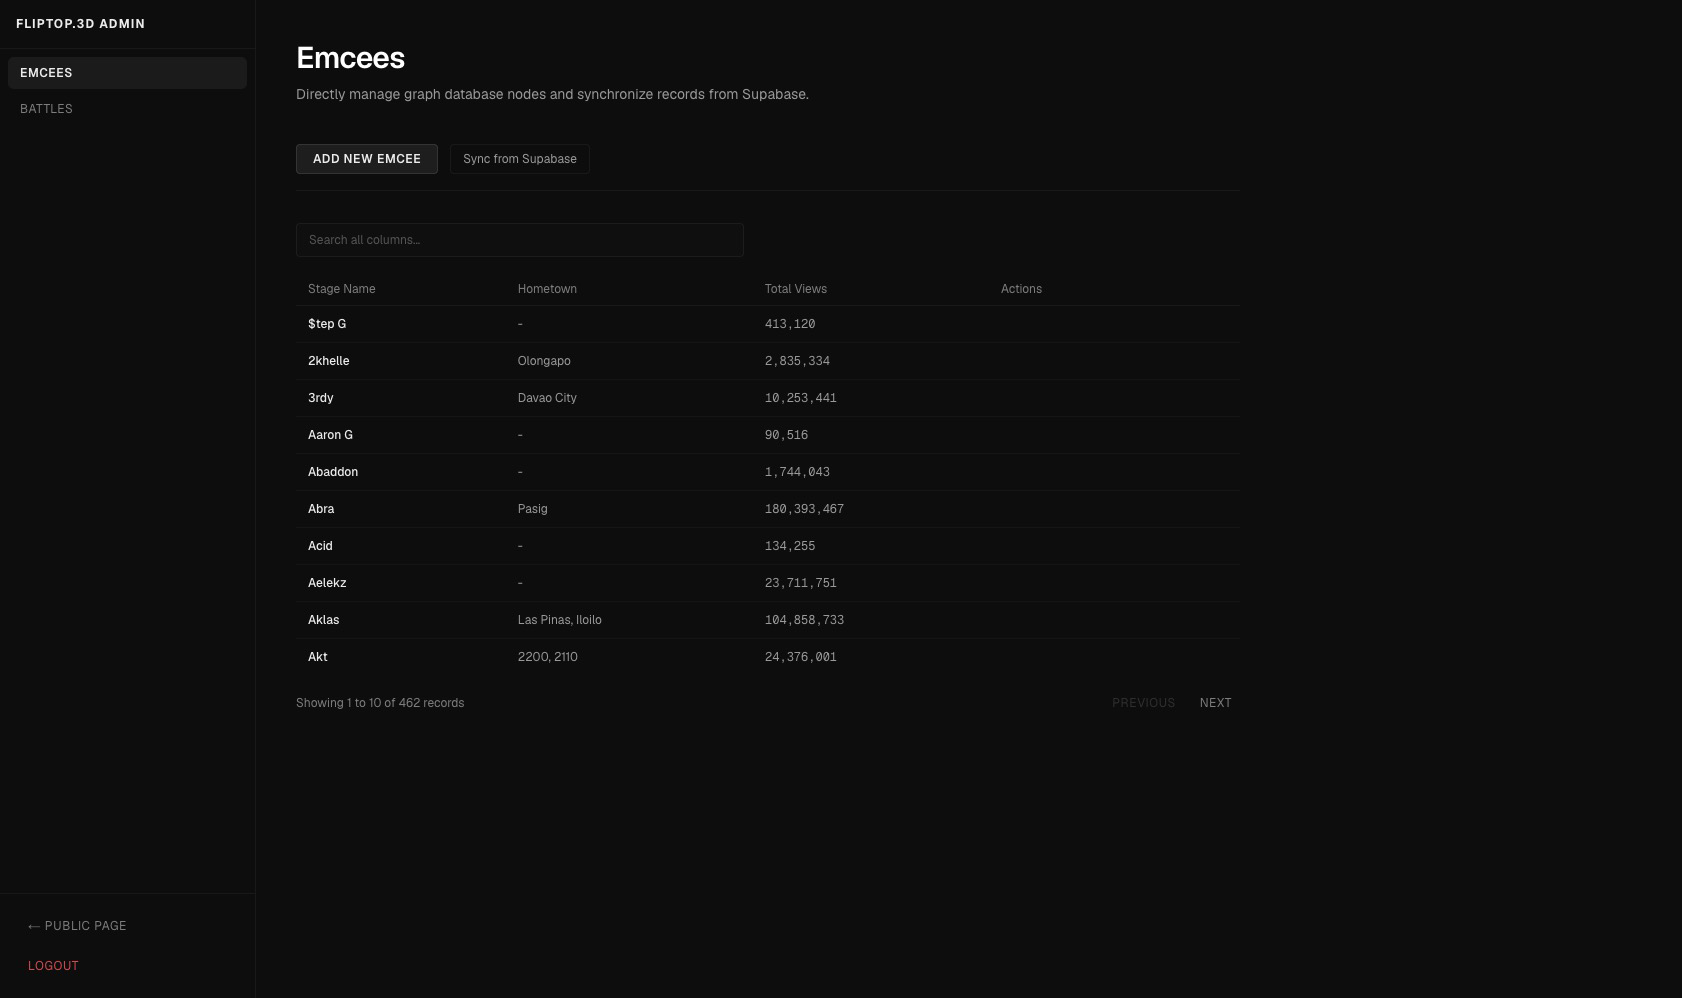
\includegraphics[width=0.8\textwidth,height=0.25\textheight,keepaspectratio]{images/admin_emcees.png}
    \caption{Admin Dashboard for Emcees (Browser: Chrome 149, OS: Mac OS Sonoma)}
    \label{fig:ui_admin_emcees}

    \vspace{0.5cm}
    
    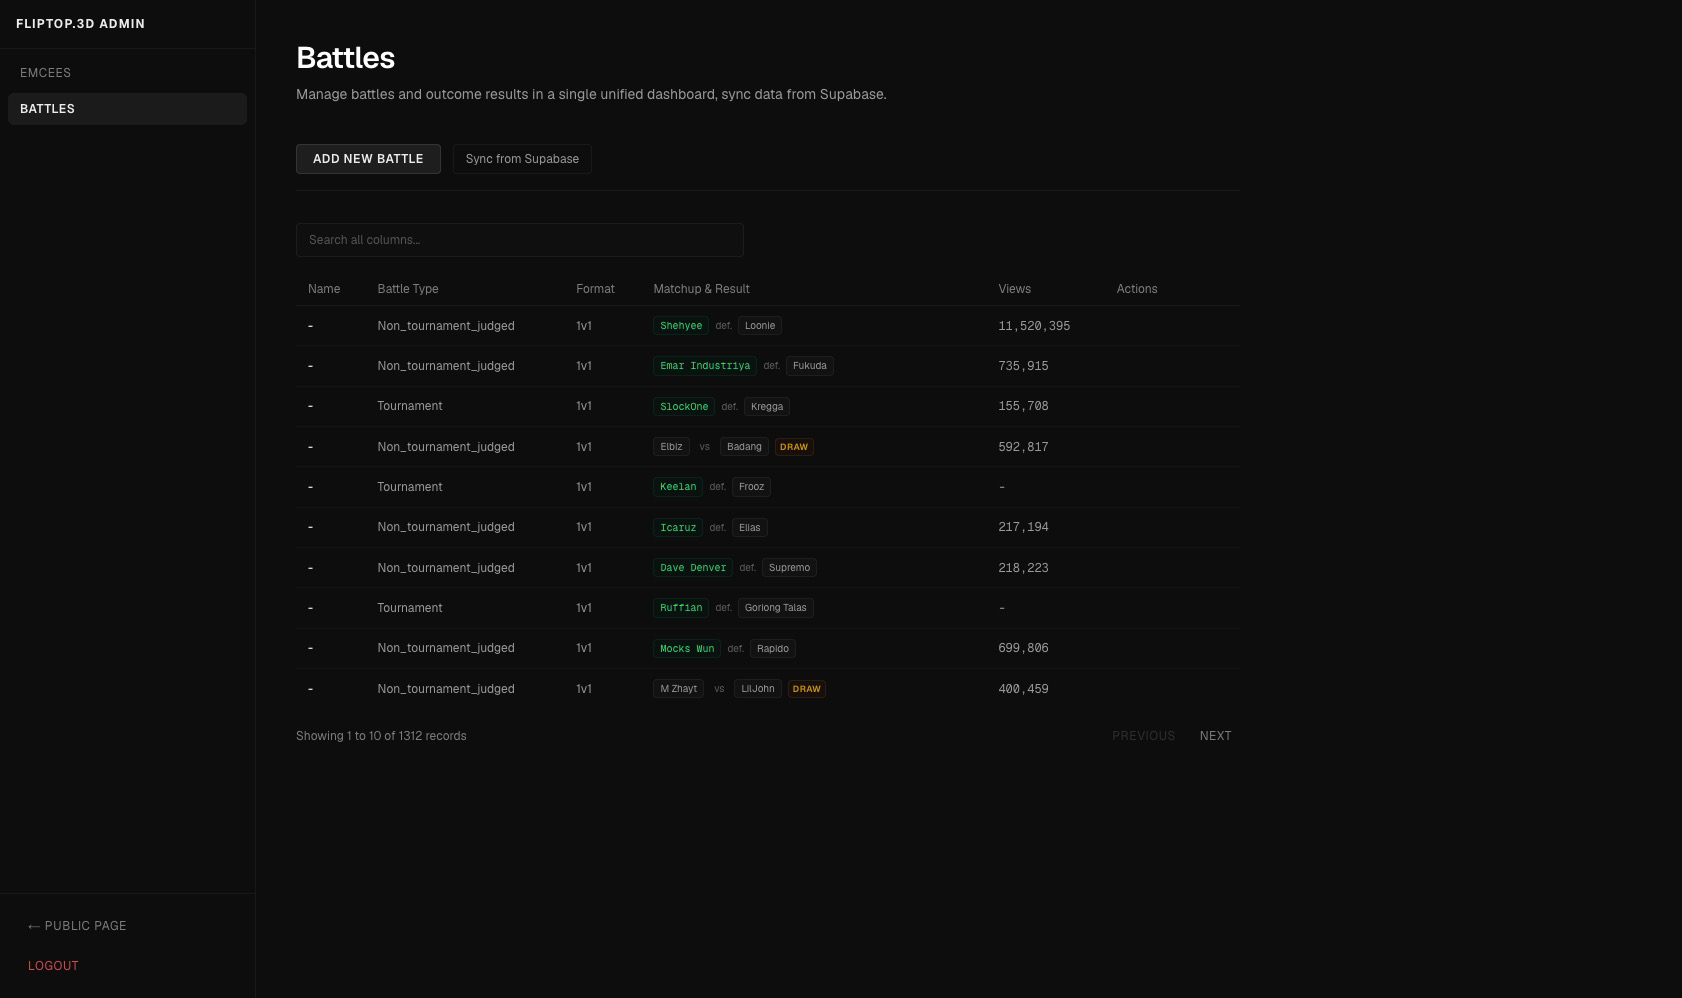
\includegraphics[width=0.8\textwidth,height=0.25\textheight,keepaspectratio]{images/admin_battles.png}
    \caption{Admin Dashboard for Battles (Browser: Chrome 149, OS: Mac OS Sonoma)}
    \label{fig:ui_admin_battles}
\end{figure}

\section{Technology Stack}

The system is built using modern, highly scalable web technologies:

\begin{itemize}
    \item \textbf{Frontend Environment:} Next.js 16 (App Router), React 19, Tailwind CSS v4.
    \item \textbf{Visualization Library:} \texttt{react-force-graph-3d} layered over Three.js.
    \item \textbf{Relational Database:} Supabase (PostgreSQL).
    \item \textbf{Graph Database:} Neo4j.
    \item \textbf{Caching Mechanism:} Upstash Redis.
\end{itemize}

\subsection{Hardware \& Software Specifications}
Due to the computationally intensive nature of mapping large datasets into physics-based 3D layouts, specific operational environments are required:
\begin{itemize}
    \item \textbf{Client Requirements:} A modern web browser (e.g., Chrome, Safari, Edge) running on a device with hardware-accelerated WebGL/GPU support to ensure smooth 60fps graph rendering. 
    \item \textbf{Server Environment:} A Node.js runtime environment capable of supporting Next.js 16 serverless execution contexts.
\end{itemize}

\section{System Limitations}
While the graph database provides a comprehensive overview of the battle rap network, it is important to note that the system accurately maps approximately 91\% of the overall results and battle data. The remaining percentage accounts for undocumented, unjudged, or lost historical footage that cannot be definitively verified.

\section{Recommendations \& Future Enhancements}
To further maximize the analytical and historical value of the \texttt{fliptop.3d} graph, several architectural and data modeling enhancements are highly recommended for future iterations:

\begin{itemize}
    \item \textbf{Expanded Entity Modeling (Judges \& Crews):} 
    \begin{itemize}
        \item \textit{Judging Bias Analysis:} Introducing ''Judge'' nodes connected via \textit{VOTED\_FOR} edges would allow the graph to visualize judging patterns, revealing whether certain judges consistently favor specific styles or specific emcees.
        \item \textit{Faction Rivalries:} Implementing ''Crew'' or ''Clan'' hyper-nodes (e.g., Uprising, Dongalo Wreckords) would enable visualizations of intra-crew alliances and large-scale inter-crew rivalries across the network's history.
    \end{itemize}
    
    \item \textbf{Data Enrichment \& Advanced Analytics:}
    \begin{itemize}
        \item \textit{Algorithmic Rankings:} Calculating and assigning Win-Loss Elo ratings or mathematical ''Impact Scores'' (PageRank) to nodes would provide a quantitative topological dominance metric, rather than relying solely on raw view counts.
        \item \textit{Metric Diversification:} Including crowd voting statistics versus official judging panel results to highlight controversial match outcomes on the graph.
    \end{itemize}
    
    \item \textbf{Advanced Temporal Visualizations:}
    \begin{itemize}
        \item \textit{Chronological Playback:} Developing a dynamic animation timeline that visually ''grows'' the 3D network year-over-year, allowing users to actively observe the physical expansion of the battle rap scene from its inception to the present day.
    \end{itemize}
    
    \item \textbf{Crowdsourcing Missing Data:}
    \begin{itemize}
        \item \textit{Community Verification Portal:} To address the current 9\% gap in historical data (due to lost or unjudged footage), the system should implement a secure, authenticated community-driven portal where super-fans can submit metadata and historical proofs to help complete the graph.
    \end{itemize}
\end{itemize}

\section{Conclusion}
The fliptop.3d system provides a highly interactive and insightful method for understanding the dense interconnected history of the Philippine battle rap scene. By strategically splitting data concerns via CQRS—utilizing PostgreSQL for administrative data integrity, Neo4j for graph relationships, and Redis for edge-cached rendering—the platform is built to be both robust and highly performant.

\begin{thebibliography}{9}

\bibitem{nextjs}
Vercel Inc. (2026). \textit{Next.js: The React Framework for the Web}. Retrieved from \url{https://nextjs.org/}

\bibitem{supabase}
Supabase Inc. (2026). \textit{Supabase: The Open Source Firebase Alternative}. Retrieved from \url{https://supabase.com/}

\bibitem{neo4j}
Neo4j, Inc. (2026). \textit{Neo4j Graph Database \& Analytics}. Retrieved from \url{https://neo4j.com/}

\bibitem{upstash}
Upstash, Inc. (2026). \textit{Upstash: Serverless Data for Redis}. Retrieved from \url{https://upstash.com/}

\bibitem{threejs}
Cabello, R., et al. (2026). \textit{Three.js: JavaScript 3D Library}. Retrieved from \url{https://threejs.org/}

\bibitem{forcegraph}
Asturiano, V. (2026). \textit{react-force-graph: React bindings for 2D/3D force-directed graphs}. Retrieved from \url{https://github.com/vasturiano/react-force-graph}

\bibitem{cqrs}
Fowler, M. (2011). \textit{CQRS (Command Query Responsibility Segregation)}. Retrieved from \url{https://martinfowler.com/bliki/CQRS.html}

\bibitem{fliptop_official}
FlipTop Battle League. (2026). \textit{Official FlipTop Website}. Retrieved from \url{https://www.fliptop.com.ph/}

\end{thebibliography}

\end{document}
